\chapter{Diseño del sistema de información}
\section{Diseño de casos de uso reales}
Esta sección presenta el diseño de los casos de uso más relevantes para el sistema. A continuación, se muestran diagramas de secuencia que ilustran las interacciones entre el usuario y los distintos componentes del sistema.
\subsection{Caso de uso: Crear cuenta}
Este caso de uso abarca todos los pasos necesarios, desde la entrada de datos por parte del usuario hasta la confirmación de la creación de la cuenta.
\\[1ex]A continuación, se detalla el flujo de interacción entre los diferentes actores y componentes del sistema mediante un diagrama de secuencia.
\begin{figure}[H]
	\centering
	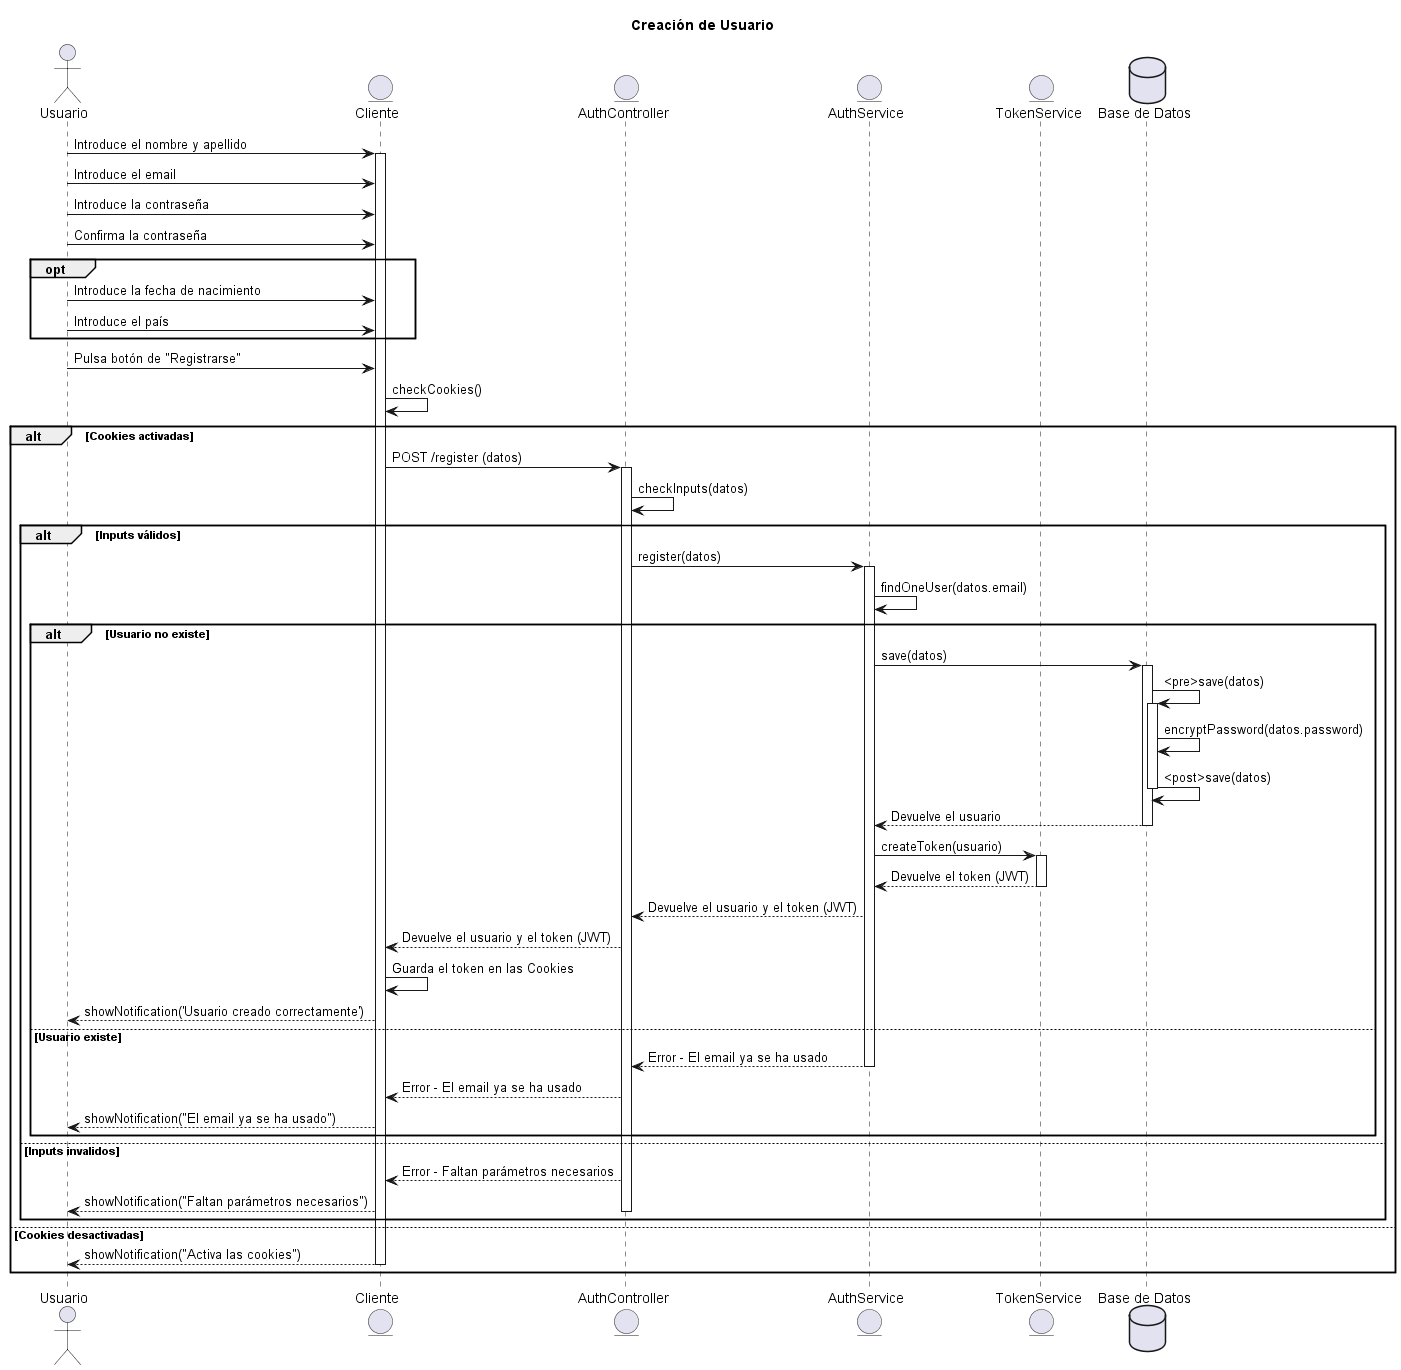
\includegraphics[width=1\linewidth]{6-DiseñoDelSistemaDeInformacion/CasosDeUso/CrearCuenta/crear-cuenta.png}
	\caption{Diagrama de secuencia: Crear cuenta.}
\end{figure}
\subsection{Caso de uso: Inicio de sesión}
Este caso de uso detalla las interacciones necesarias entre el usuario y los componentes del sistema para autenticar al usuario de manera segura y eficiente.
\\[1ex]A continuación, se presenta el diagrama de secuencia que describe estas interacciones.
\begin{figure}[H]
	\centering
	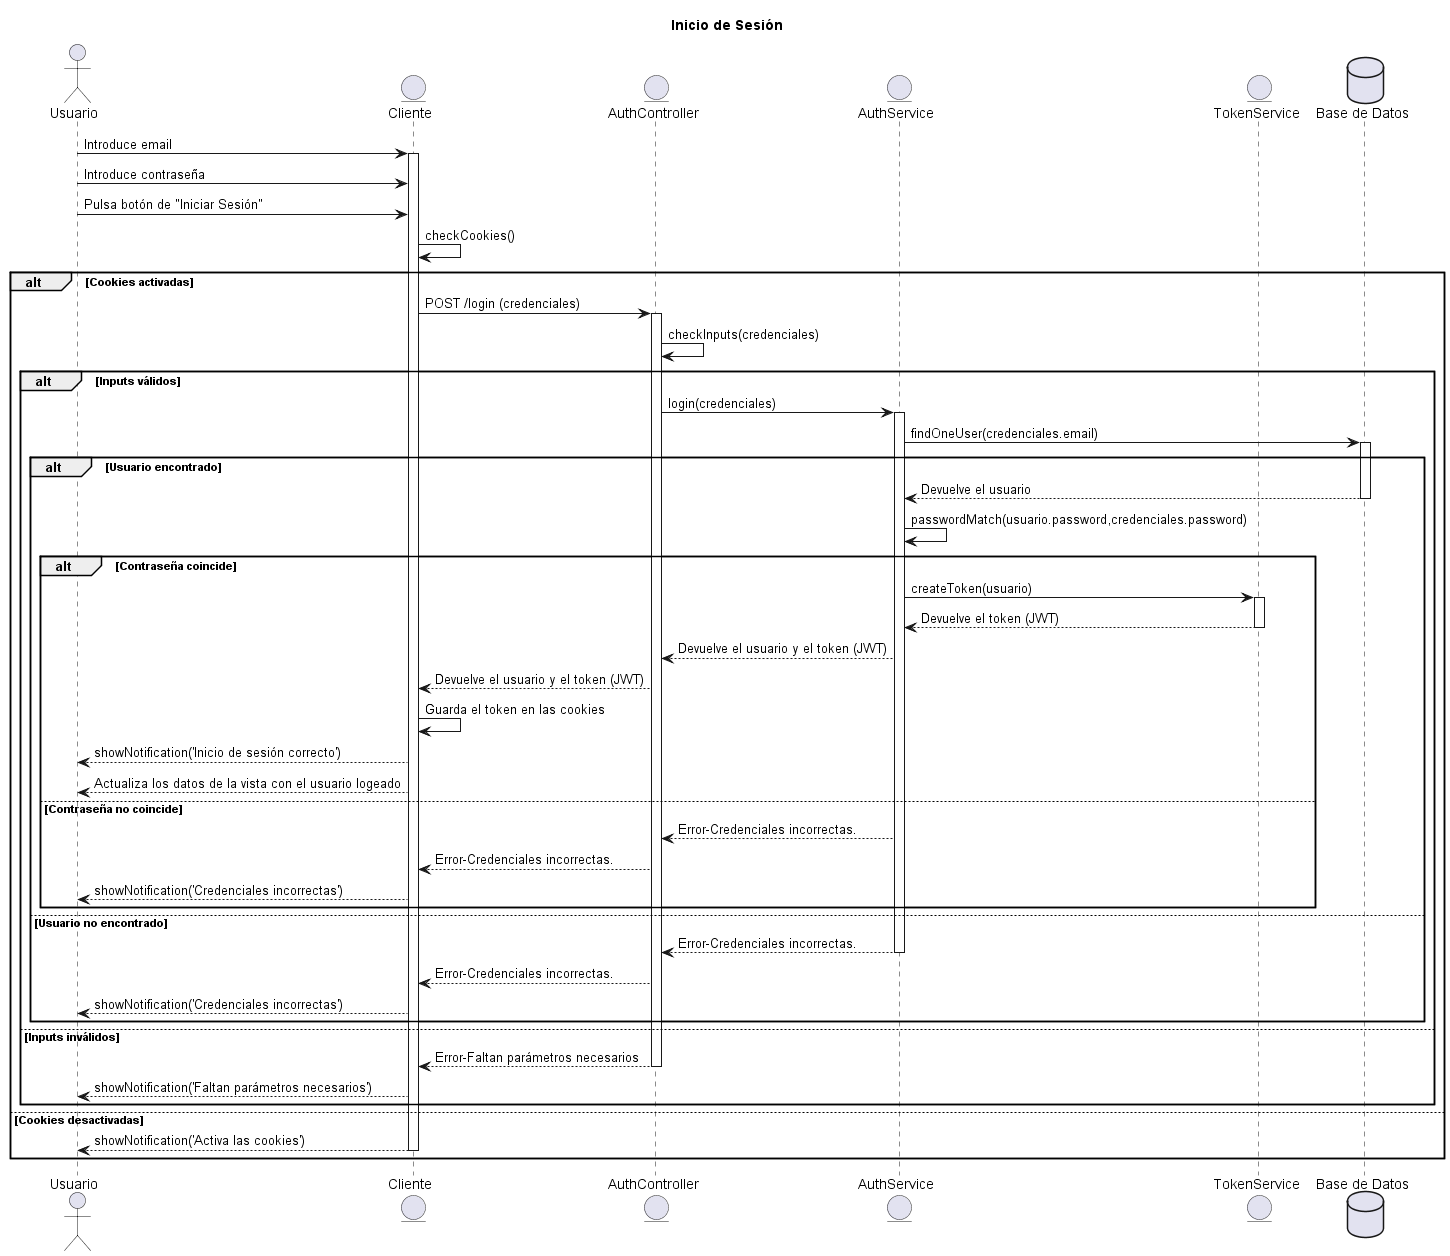
\includegraphics[width=1\linewidth]{6-DiseñoDelSistemaDeInformacion/CasosDeUso/InicioDeSesion/inicio-de-sesion.png}
	\caption{Diagrama de secuencia: Inicio de sesión.}
\end{figure}
\subsection{Caso de uso: Buscar actividades}
Este caso de uso describe las interacciones necesarias para que el usuario pueda buscar actividades en la aplicación.
\\[1ex]A continuación, se presenta el diagrama de secuencia que describe estas interacciones.
\begin{figure}[H]
	\centering
	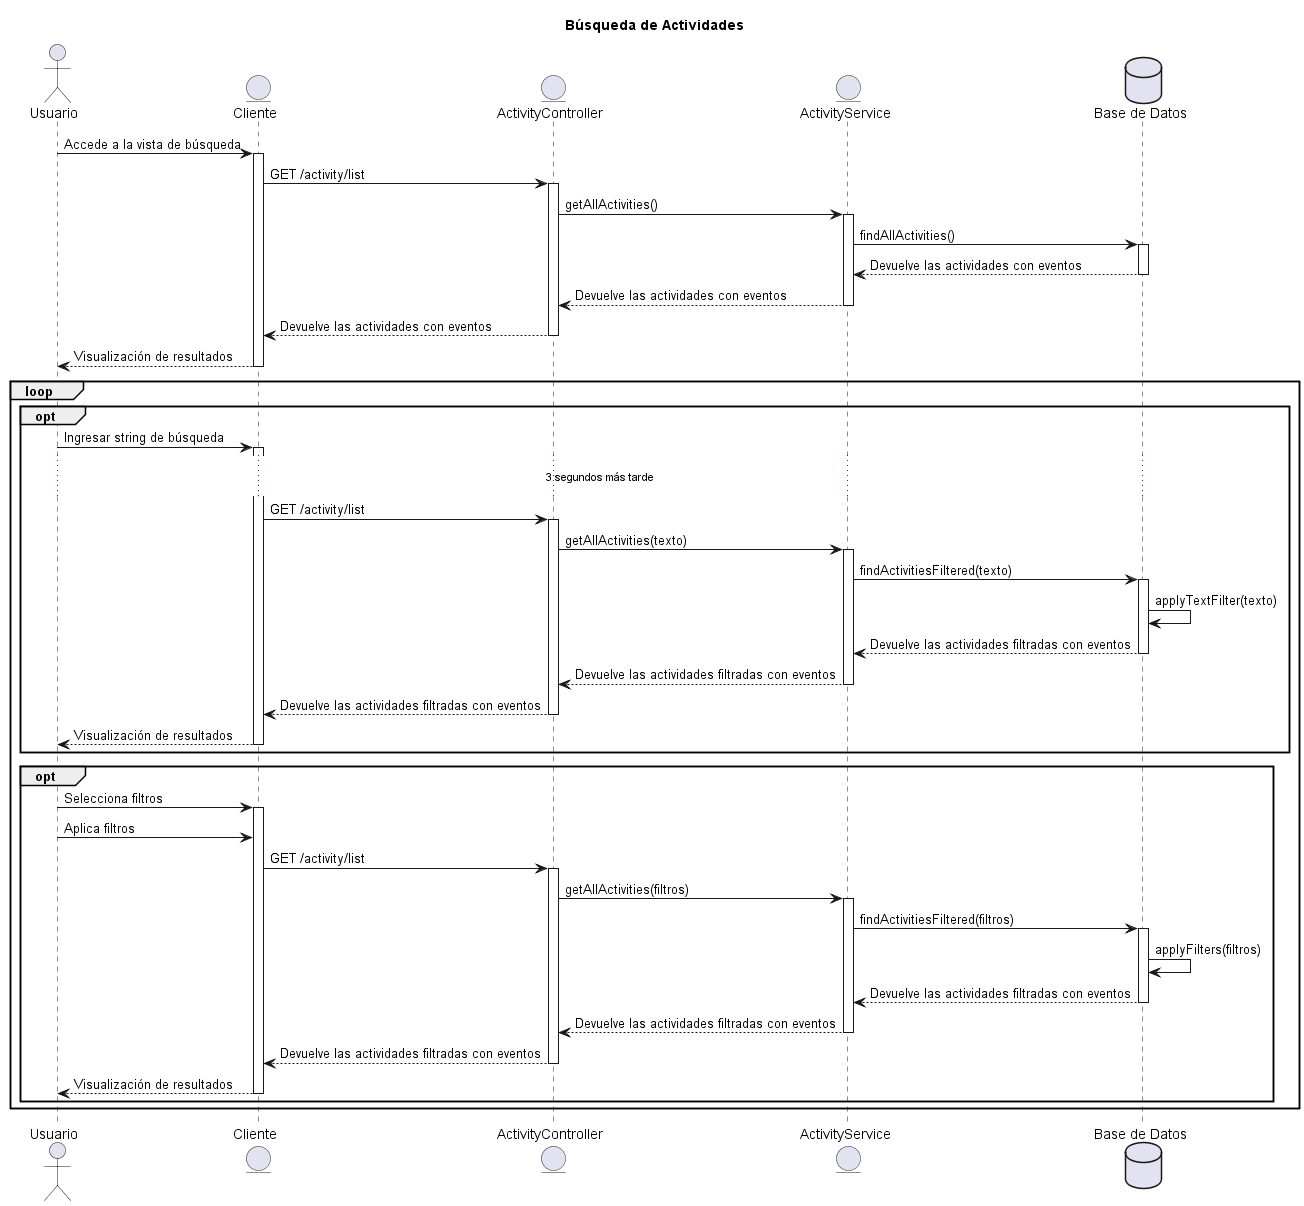
\includegraphics[width=1\linewidth]{6-DiseñoDelSistemaDeInformacion/CasosDeUso/BuscarActividades/buscar-actividades.png}
	\caption{Diagrama de secuencia: Buscar actividades.}
\end{figure}
\subsection{Caso de uso: Crear una reserva}
Este caso de uso muestra las interacciones necesarias para que el usuario pueda realizar una reserva en la aplicación.
\\[1ex]A continuación, se presenta el diagrama de secuencia que describe estas interacciones.
\begin{figure}[H]
	\centering
	\begin{adjustwidth}{-0.7cm}{}
		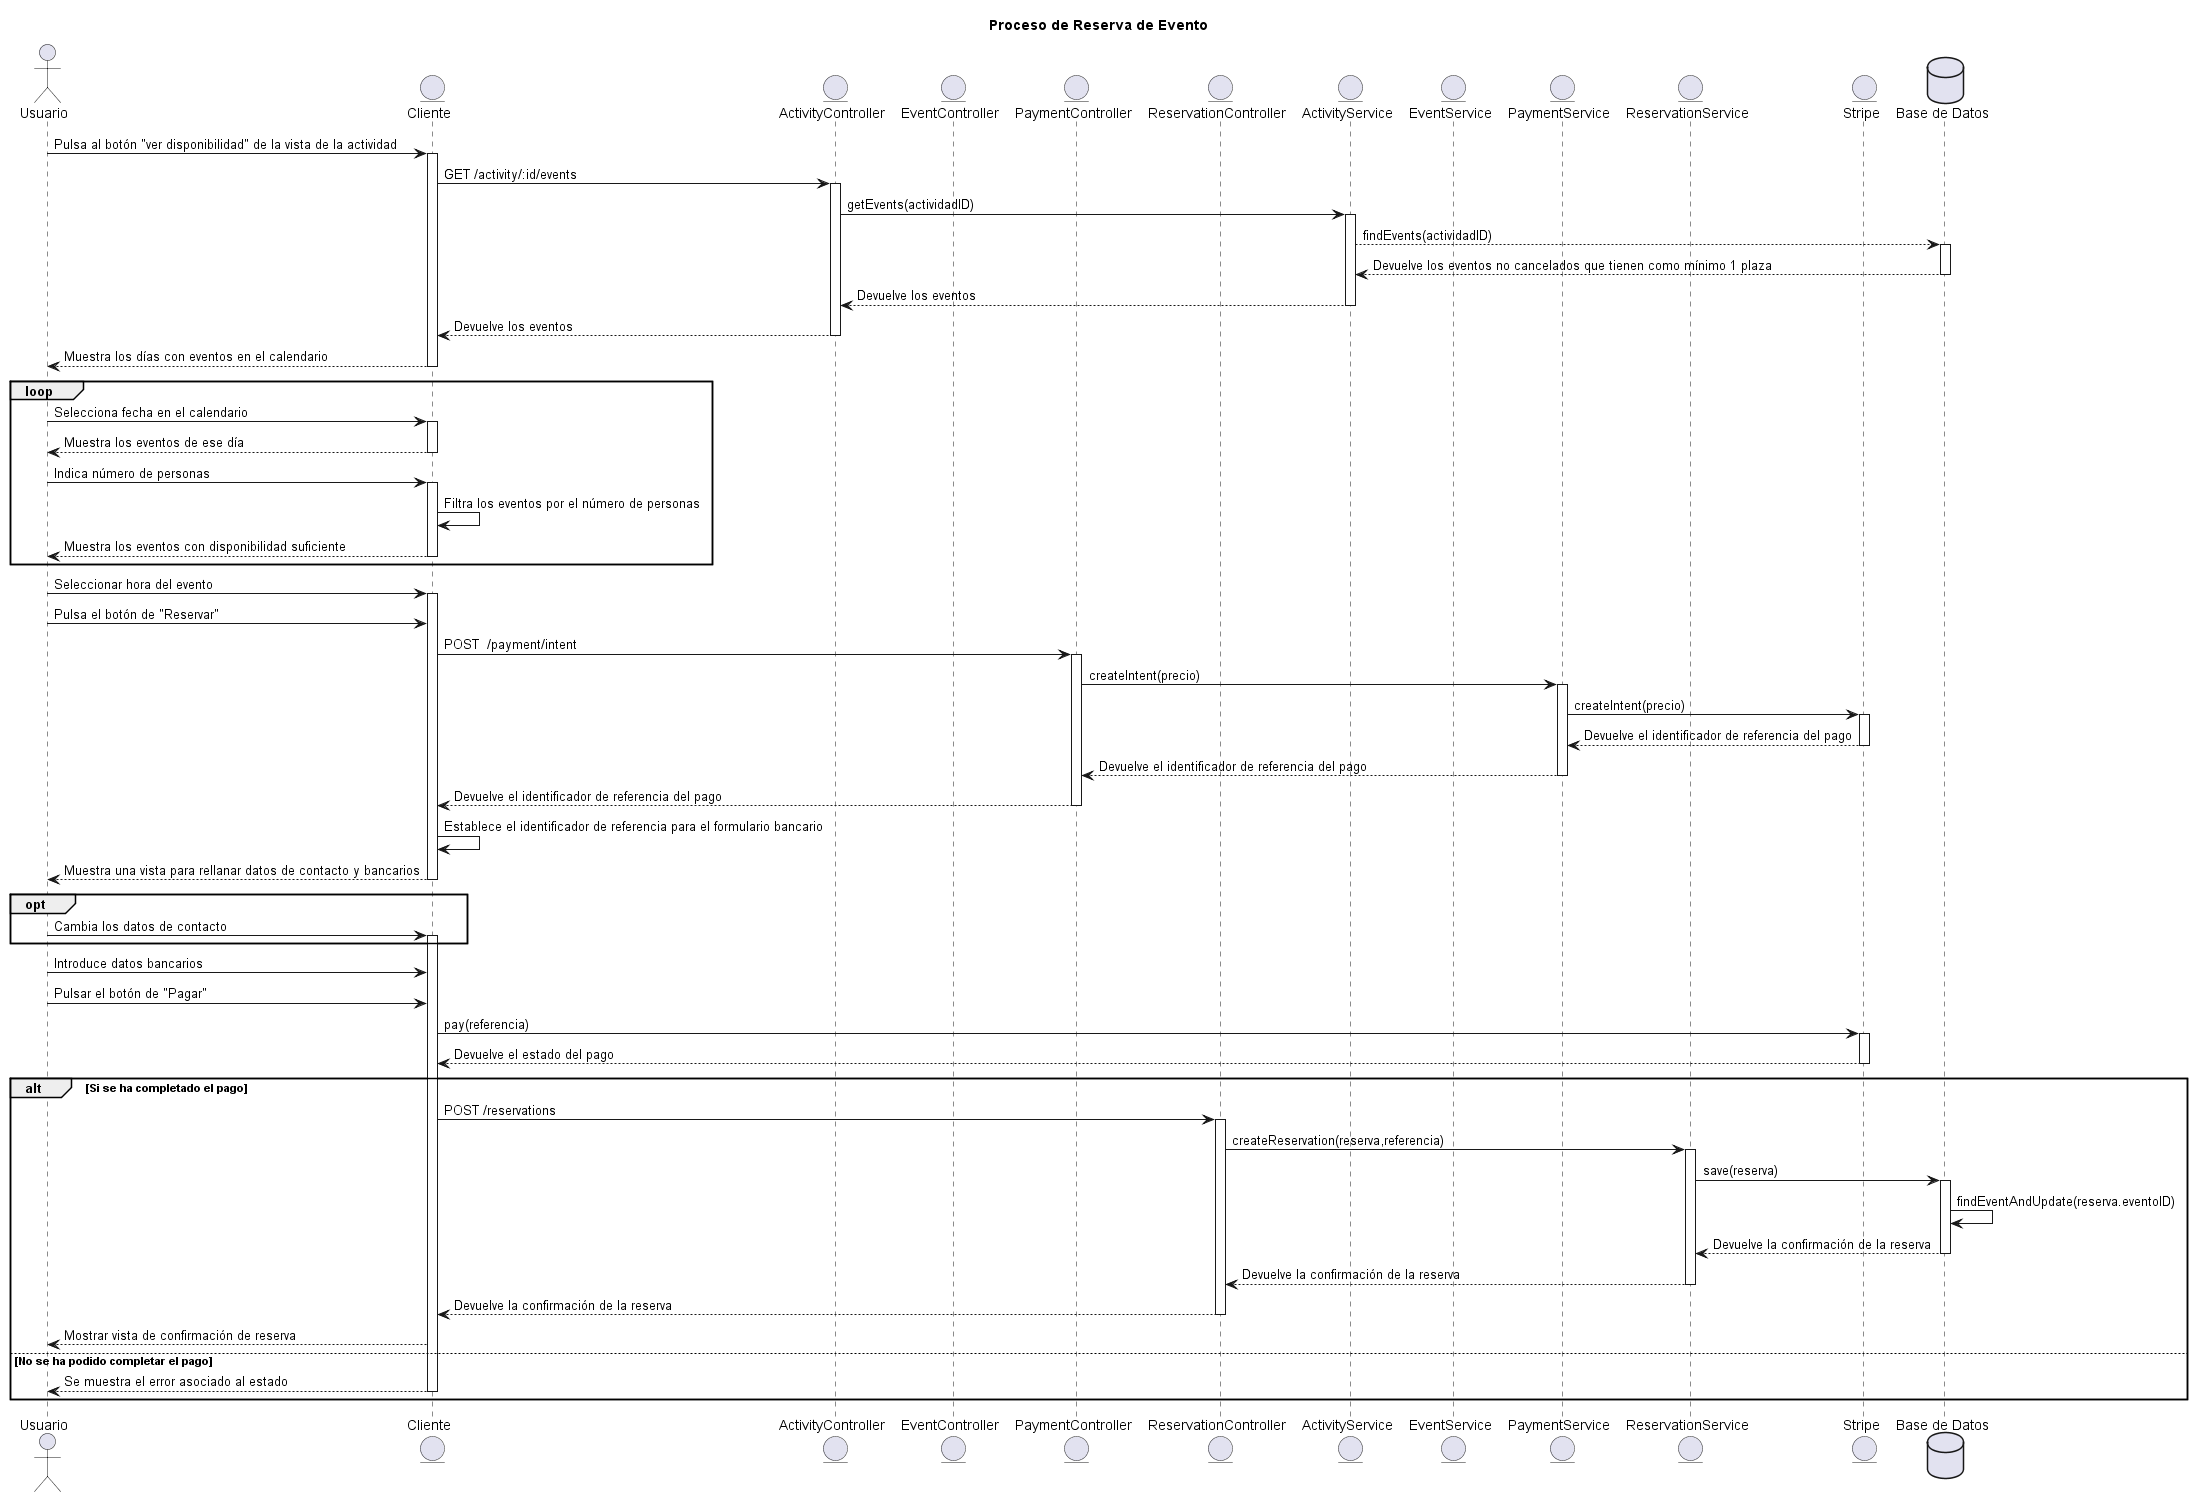
\includegraphics[width=1.05\linewidth]{6-DiseñoDelSistemaDeInformacion/CasosDeUso/CrearReserva/crear-reserva.png}
	\end{adjustwidth}
	\caption{Diagrama de secuencia: Crear reserva.}
\end{figure}

% \subsubsection{Diagrama de estados}
% \begin{figure}[H]
	\centering
	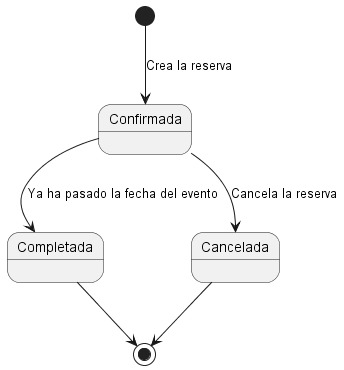
\includegraphics[width=1.05\linewidth]{6-DiseñoDelSistemaDeInformacion/CasosDeUso/CrearReserva/estados-reserva.png}
	\caption{Diagrama de estados: Reserva.}
\end{figure}
\section{Diseño de clases}
\subsection{Diagrama de clases}
\input{6-DiseñoDelSistemaDeInformacion/diagrama-de-clases.tex}
\section{Diseño de la arquitectura de módulos del sistema}
\subsection{Diseño de módulos del sistema}
\subsubsection{Módulo del cliente}
El módulo del cliente se compone de varios paquetes esenciales, cada uno con un rol específico en la estructura del sistema:
\begin{itemize}
	\item \textbf{Componentes:}  Este paquete contiene todos los componentes de la interfaz de usuario que se componen para formar las diferentes vistas de la aplicación.
	\item \textbf{Layouts:} Define la estructura general de las páginas, utilizando componentes y temas para asegurar una apariencia consistente en toda la aplicación.
	\item \textbf{Tema:} Se utiliza para aplicar estilos y temas consistentes a los componentes y layouts, asegurando una experiencia de usuario uniforme.
	\item \textbf{Hooks:} Almacena la lógica reutilizable que puede ser compartida entre diferentes componentes. Utiliza APIs y contextos para manejar datos y estados.
	\item \textbf{APIs:} Gestiona la comunicación con el servidor, realizando llamadas a las diferentes APIs necesarias para la funcionalidad de la aplicación.
	\item \textbf{Contextos:} Proporciona un mecanismo para compartir estados y datos entre componentes sin necesidad de pasar props manualmente en cada nivel.
\end{itemize}
El diagrama también muestra cómo el cliente se comunica con el servidor, asegurando que los datos fluyan correctamente entre el frontend y el backend.

\begin{figure}[H]
	\centering
	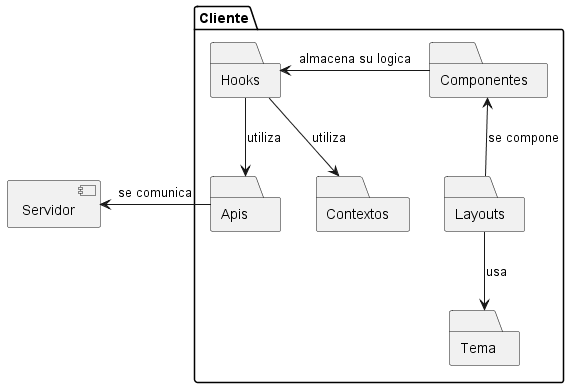
\includegraphics[width=1\linewidth]{6-DiseñoDelSistemaDeInformacion/Modulos/cliente.png}
	\caption{Diagrama de paquetes del Cliente}
\end{figure}
\subsubsection{Módulo del servidor}
El módulo del servidor se encarga de gestionar la lógica de negocio y la comunicación con la base de datos. A continuación, se presenta el diagrama de paquetes del servidor, que muestra la organización de sus componentes y la interacción entre ellos.
\\[1ex]
El servidor está compuesto por los siguientes paquetes:
\begin{itemize}
	\item \textbf{API:} Define la interfaz de comunicación entre el cliente y el servidor, especificando los endpoints disponibles.
	\item \textbf{Rutas:} Maneja la definición y el manejo de las rutas que el servidor expone, asociando cada ruta a su controlador correspondiente.
	\item \textbf{Middlewares:} Aplica funciones intermedias en la cadena de solicitudes HTTP, como autenticación, validación de datos y manejo de errores.
	\item \textbf{Controladores:} Contienen la lógica que maneja las solicitudes del cliente, delegando tareas específicas a los servicios y middlewares.
	\item \textbf{Servicios:} Implementan la lógica de negocio, realizando operaciones complejas y coordinando la interacción entre controladores y modelos.
	\item \textbf{Modelos:} Interactúan con la base de datos, definiendo la estructura de los datos y proporcionando métodos para su manipulación.
\end{itemize}

El diagrama también muestra cómo el cliente se comunica con la API del servidor y cómo el servidor maneja las solicitudes a través de sus componentes hasta llegar a la base de datos y viceversa.

\begin{figure}[H]
	\centering
	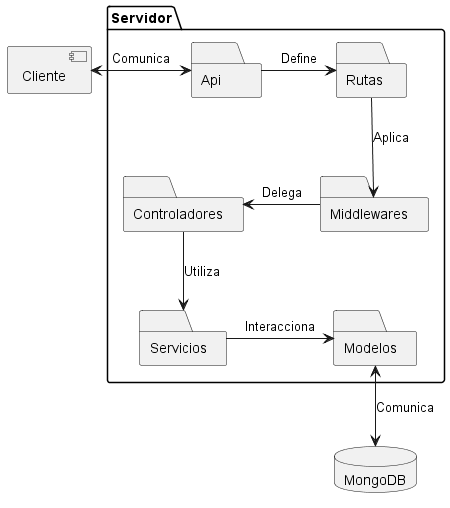
\includegraphics[width=1\linewidth]{6-DiseñoDelSistemaDeInformacion/Modulos/servidor.png}
	\caption{Diagrama de paquetes del Servidor}
\end{figure}
\subsection{Diseño de comunicaciones entre módulos}
\subsubsection{Diagrama de despliegue}
El diagrama de despliegue ilustra la arquitectura de la comunicación entre los módulos del sistema, destacando las conexiones y protocolos utilizados:
\begin{itemize}
	\item \textbf{Usuario:} Los usuarios acceden al sistema a través de dispositivos que pueden ser aplicaciones móviles (App) o navegadores web (Browser). La comunicación se realiza mediante el protocolo HTTPS en el puerto 443 para garantizar la seguridad de los datos transmitidos.
	\item \textbf{Servidor Web:} Este componente, desplegado en la nube, aloja la página web de la aplicación. Se encarga de servir las interfaces de usuario y manejar las solicitudes HTTPS provenientes de los clientes.
	\item \textbf{Servidor (AWS EC2):} El servidor principal está desplegado en un servicio EC2 de AWS. Este servidor maneja la lógica de negocio y procesa las solicitudes de los usuarios, comunicándose con la base de datos para acceder y manipular la información necesaria.
	\item \textbf{Base de Datos (MongoDB Atlas):} La base de datos está alojada en MongoDB Atlas, un servicio de base de datos en la nube. Este componente almacena todos los datos del sistema, organizados en esquemas como “Actividades” y “Usuarios”. La comunicación entre el servidor y la base de datos se realiza a través de una URI segura.
\end{itemize}

El diagrama también muestra cómo el servidor web y el servidor principal (EC2) se comunican con la base de datos en MongoDB Atlas.

\begin{figure}[H]
	\centering
	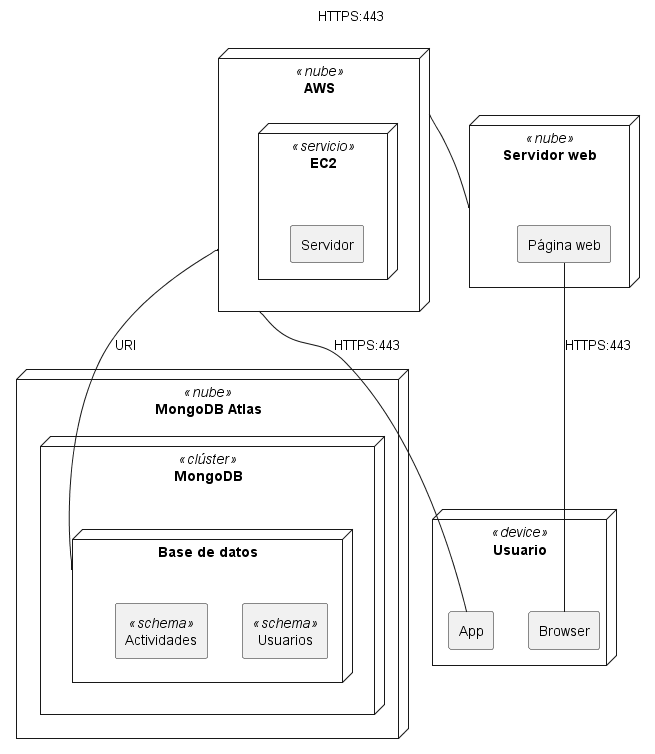
\includegraphics[width=1\linewidth]{6-DiseñoDelSistemaDeInformacion/Modulos/comunicaciones.png}
	\caption{Diagrama de despliegue}
\end{figure}

\section{Revisión de la interfaz de usuario}
\subsubsection{Inicio}
La vista “Inicio” será aquella que se vea nada más acceder a la aplicación. En ella se pondrá observar la lista de actividades más populares así como un botón para poder ir directamente a la búsqueda de actividades.
\begin{figure}[H]
	\centering
	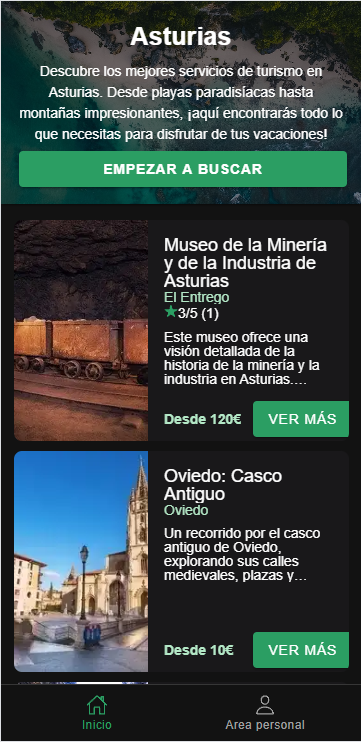
\includegraphics[width=0.18\textwidth]{6-DiseñoDelSistemaDeInformacion/RevisionInterfaces/Inicio/inicio-admin-app.png}
	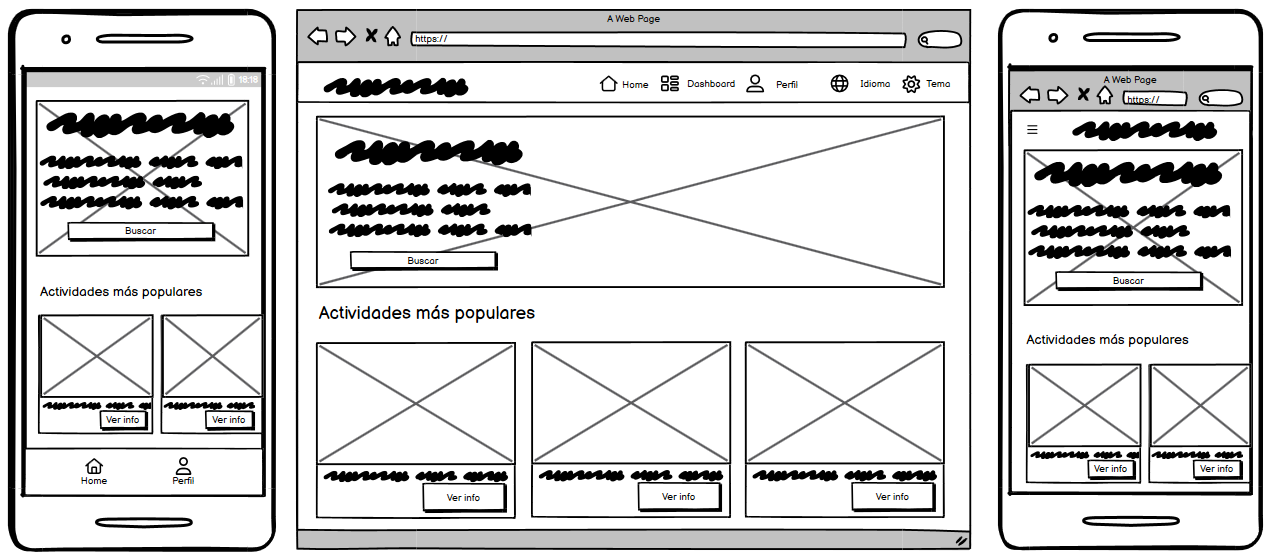
\includegraphics[width=0.5\textwidth]{6-DiseñoDelSistemaDeInformacion/RevisionInterfaces/Inicio/inicio-admin.png}
	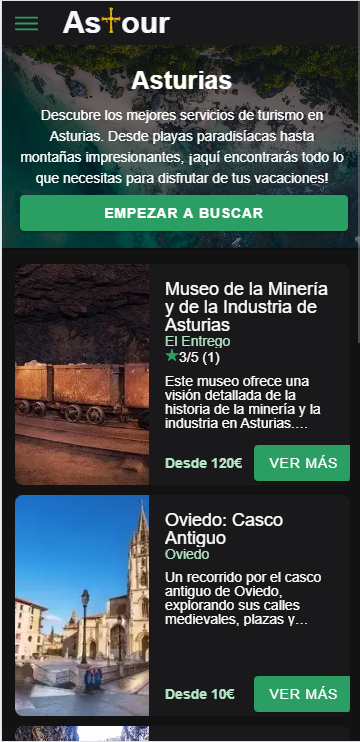
\includegraphics[width=0.18\textwidth]{6-DiseñoDelSistemaDeInformacion/RevisionInterfaces/Inicio/inicio-admin-mobile.png}
	\caption{Inicio - Vista Administrador }
\end{figure}

\begin{figure}[H]
	\centering
	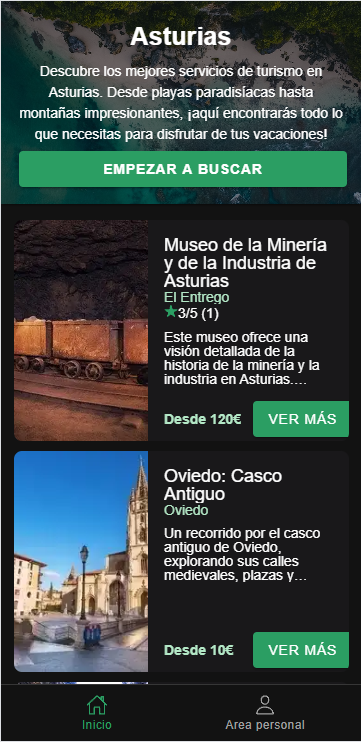
\includegraphics[width=0.18\textwidth]{6-DiseñoDelSistemaDeInformacion/RevisionInterfaces/Inicio/inicio-admin-app.png}
	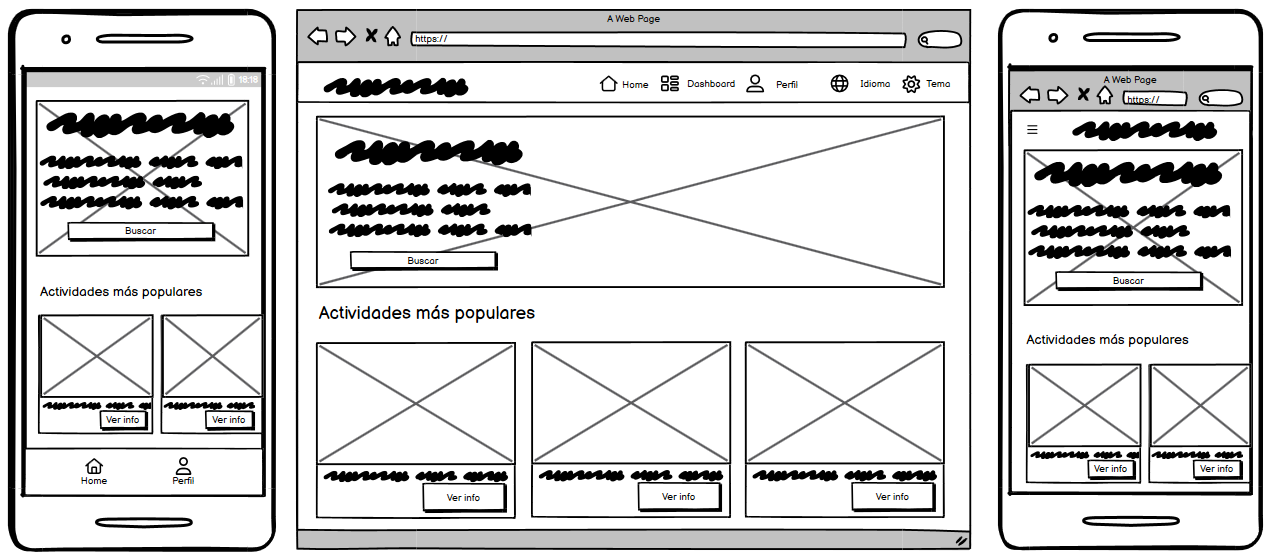
\includegraphics[width=0.5\textwidth]{6-DiseñoDelSistemaDeInformacion/RevisionInterfaces/Inicio/inicio-admin.png}
	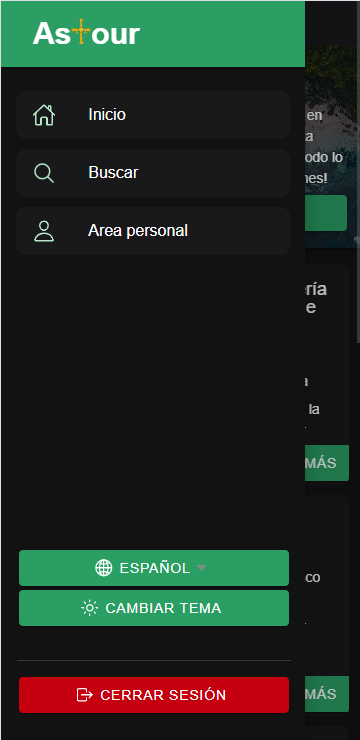
\includegraphics[width=0.18\textwidth]{6-DiseñoDelSistemaDeInformacion/RevisionInterfaces/Inicio/inicio-admin-menu.png}
	\caption{Inicio - Vista Administrador (Menú desplegado)}
\end{figure}

\begin{figure}[H]
	\centering
	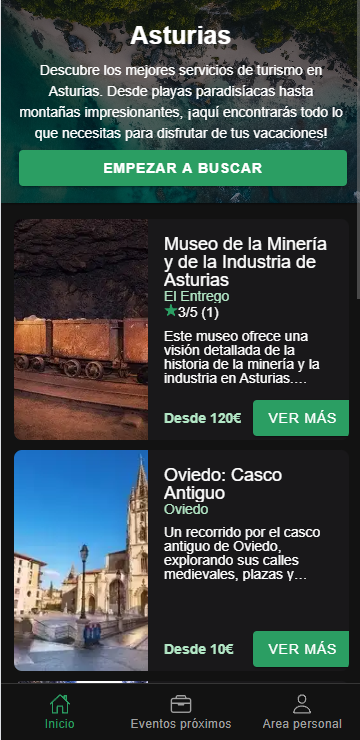
\includegraphics[width=0.18\textwidth]{6-DiseñoDelSistemaDeInformacion/RevisionInterfaces/Inicio/inicio-guia-app.png}
	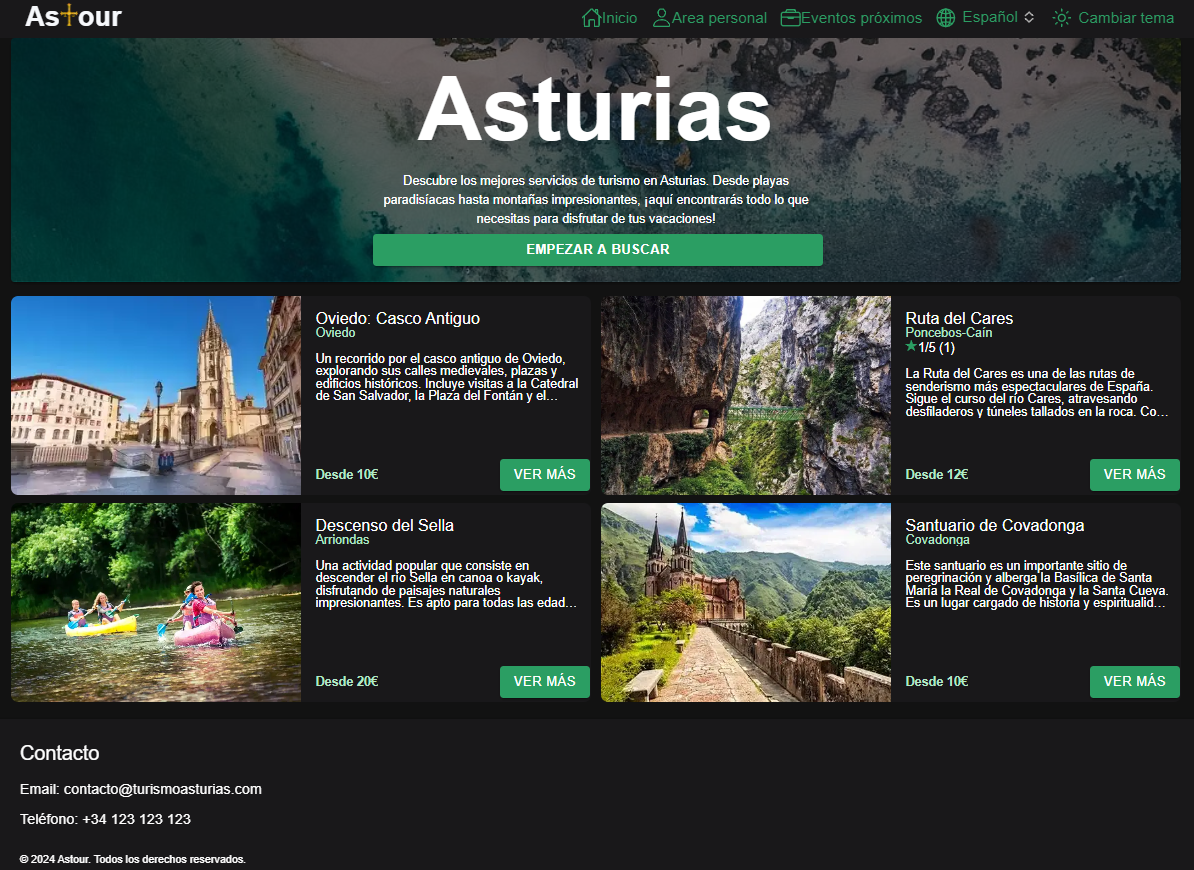
\includegraphics[width=0.5\textwidth]{6-DiseñoDelSistemaDeInformacion/RevisionInterfaces/Inicio/inicio-guia.png}
	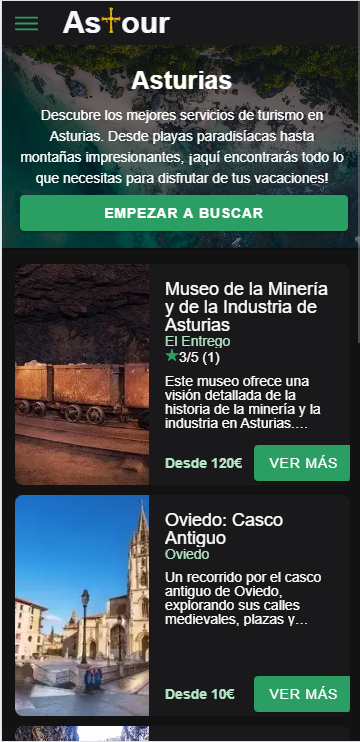
\includegraphics[width=0.18\textwidth]{6-DiseñoDelSistemaDeInformacion/RevisionInterfaces/Inicio/inicio-admin-mobile.png}
	\caption{Inicio - Vista Guía }
\end{figure}

\begin{figure}[H]
	\centering
	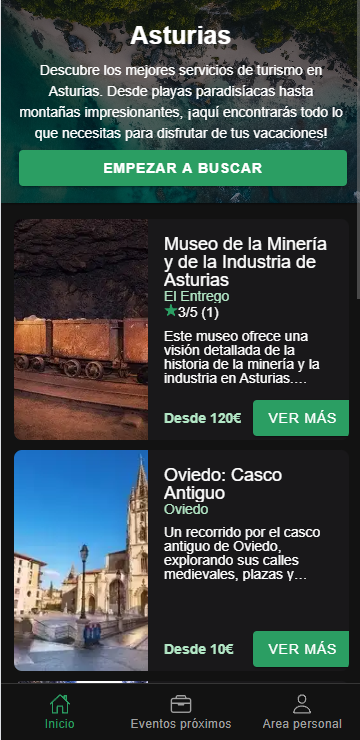
\includegraphics[width=0.18\textwidth]{6-DiseñoDelSistemaDeInformacion/RevisionInterfaces/Inicio/inicio-guia-app.png}
	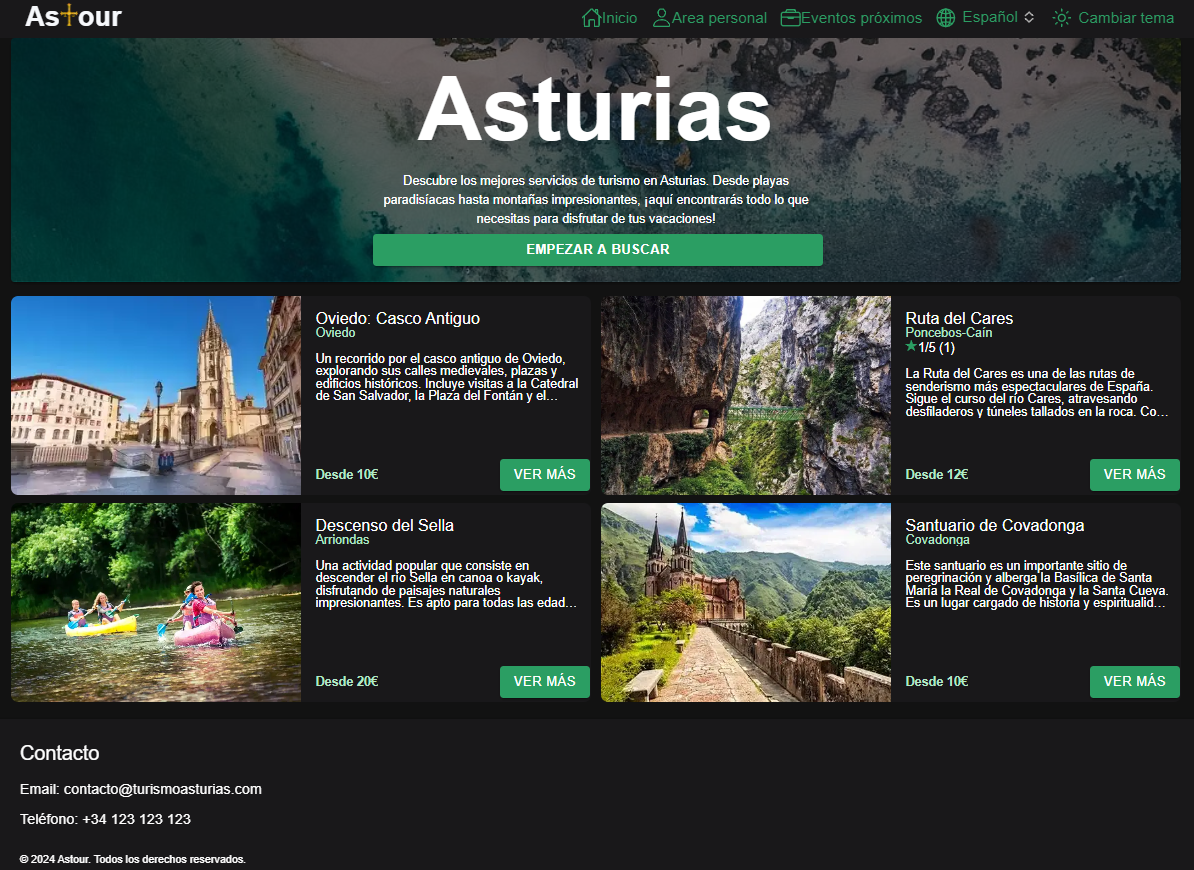
\includegraphics[width=0.5\textwidth]{6-DiseñoDelSistemaDeInformacion/RevisionInterfaces/Inicio/inicio-guia.png}
	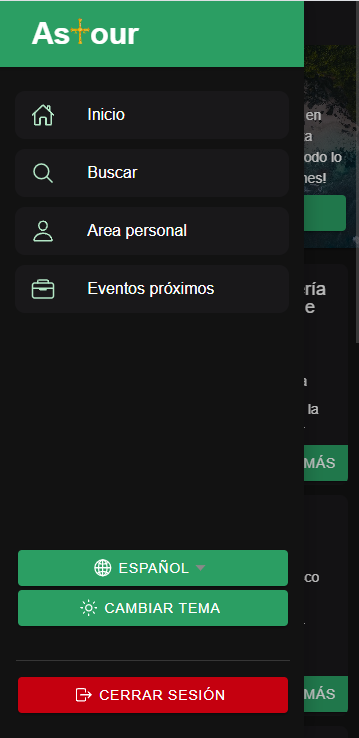
\includegraphics[width=0.18\textwidth]{6-DiseñoDelSistemaDeInformacion/RevisionInterfaces/Inicio/inicio-guia-menu.png}
	\caption{Inicio - Vista Guía (Menú desplegado)}
\end{figure}

\begin{figure}[H]
	\centering
	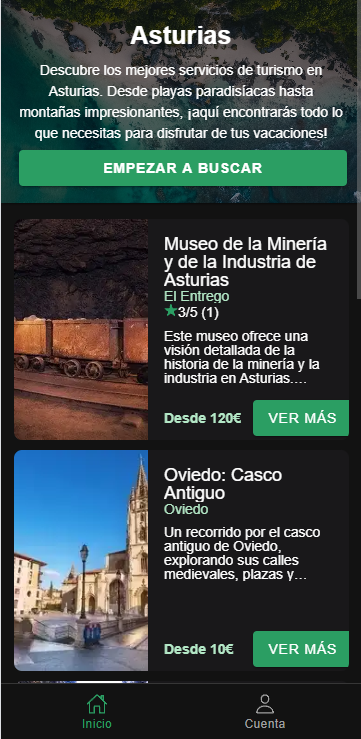
\includegraphics[width=0.18\textwidth]{6-DiseñoDelSistemaDeInformacion/RevisionInterfaces/Inicio/inicio-no-identificado-app.png}
	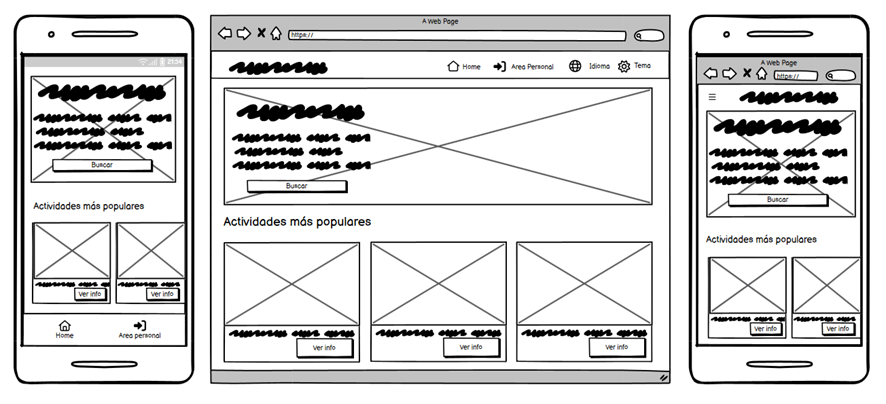
\includegraphics[width=0.5\textwidth]{6-DiseñoDelSistemaDeInformacion/RevisionInterfaces/Inicio/inicio-no-identificado.png}
	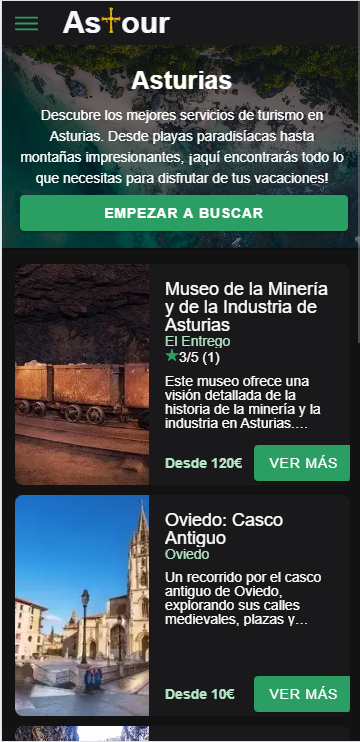
\includegraphics[width=0.18\textwidth]{6-DiseñoDelSistemaDeInformacion/RevisionInterfaces/Inicio/inicio-admin-mobile.png}
	\caption{Inicio - Vista Usuario no identificado }
\end{figure}

\begin{figure}[H]
	\centering
	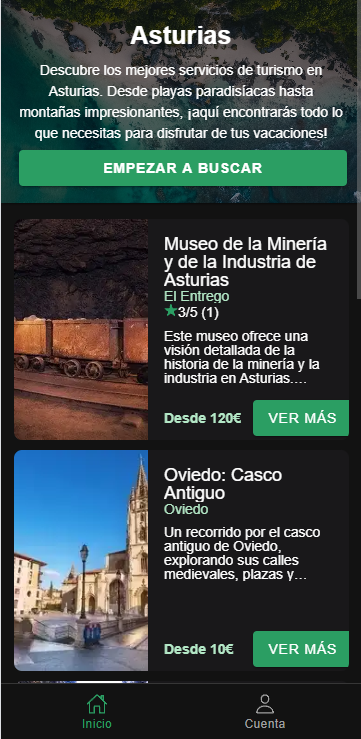
\includegraphics[width=0.18\textwidth]{6-DiseñoDelSistemaDeInformacion/RevisionInterfaces/Inicio/inicio-no-identificado-app.png}
	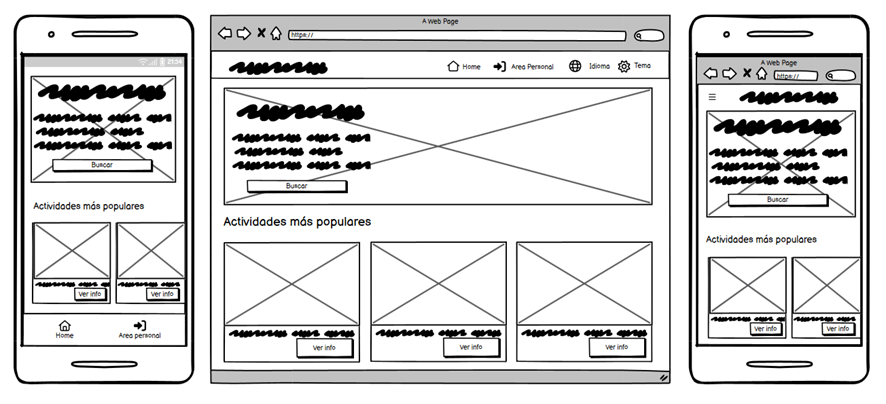
\includegraphics[width=0.5\textwidth]{6-DiseñoDelSistemaDeInformacion/RevisionInterfaces/Inicio/inicio-no-identificado.png}
	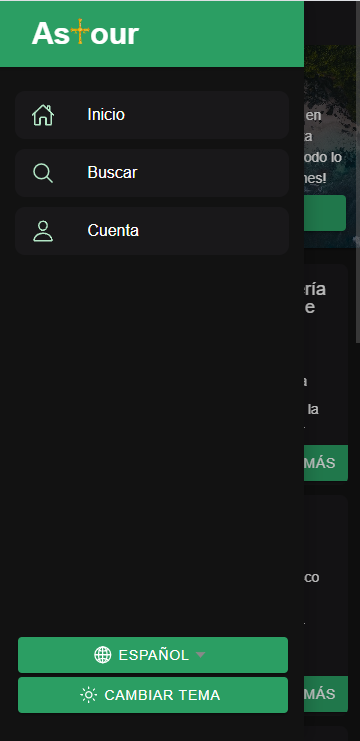
\includegraphics[width=0.18\textwidth]{6-DiseñoDelSistemaDeInformacion/RevisionInterfaces/Inicio/inicio-no-identificado-menu.png}
	\caption{Inicio - Vista Usuario no identificado (Menú desplegado)}
\end{figure}

\begin{figure}[H]
	\centering
	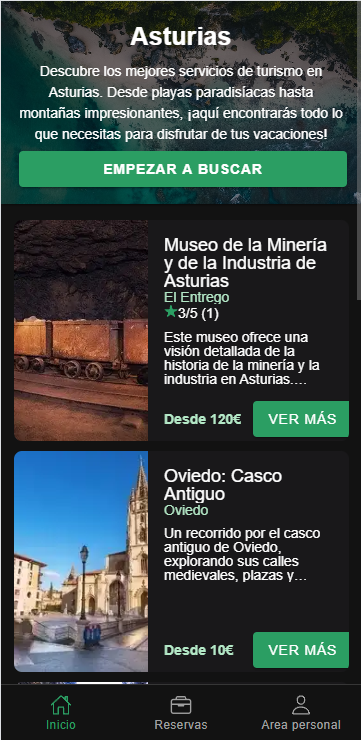
\includegraphics[width=0.18\textwidth]{6-DiseñoDelSistemaDeInformacion/RevisionInterfaces/Inicio/inicio-turista-app.png}
	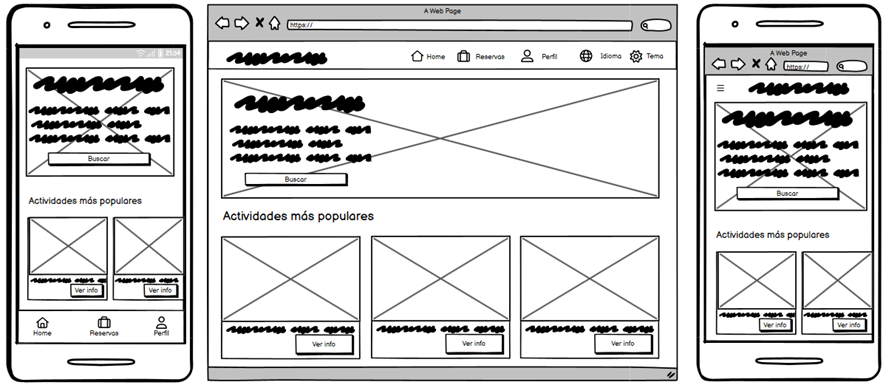
\includegraphics[width=0.5\textwidth]{6-DiseñoDelSistemaDeInformacion/RevisionInterfaces/Inicio/inicio-turista.png}
	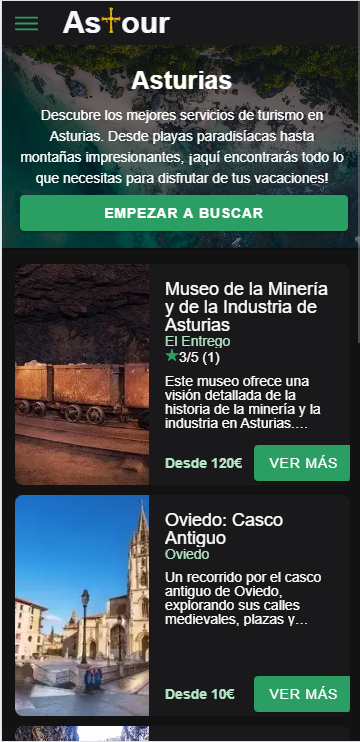
\includegraphics[width=0.18\textwidth]{6-DiseñoDelSistemaDeInformacion/RevisionInterfaces/Inicio/inicio-admin-mobile.png}
	\caption{Inicio - Vista Turista }
\end{figure}

\begin{figure}[H]
	\centering
	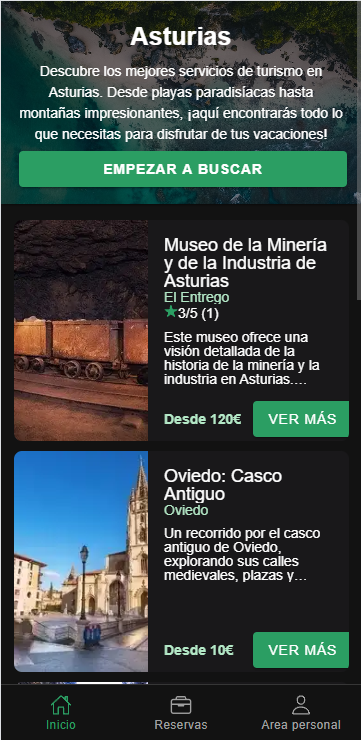
\includegraphics[width=0.18\textwidth]{6-DiseñoDelSistemaDeInformacion/RevisionInterfaces/Inicio/inicio-turista-app.png}
	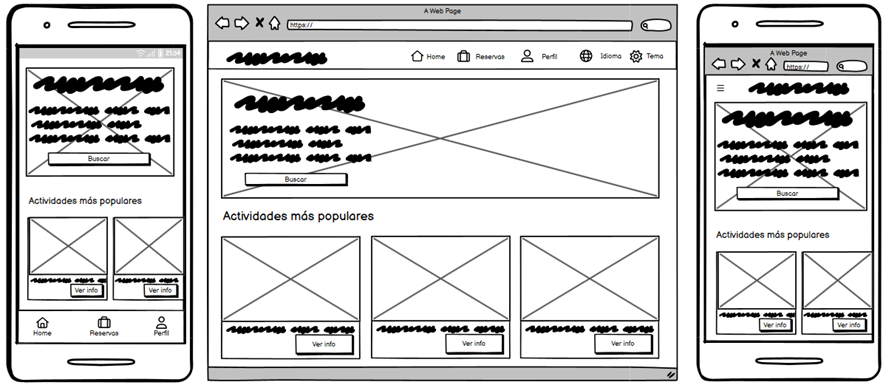
\includegraphics[width=0.5\textwidth]{6-DiseñoDelSistemaDeInformacion/RevisionInterfaces/Inicio/inicio-turista.png}
	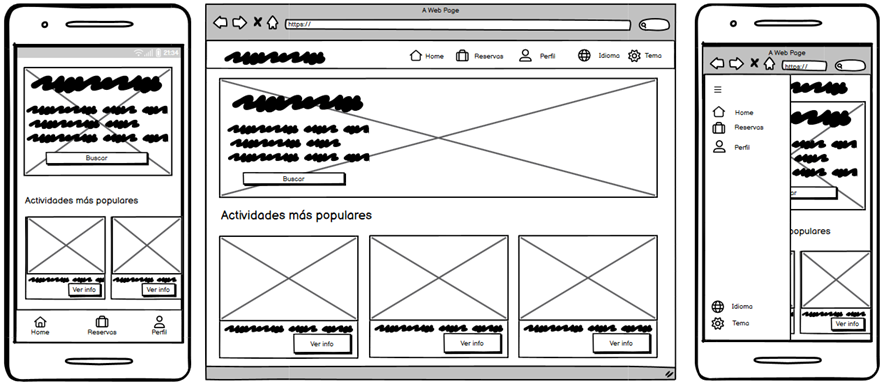
\includegraphics[width=0.18\textwidth]{6-DiseñoDelSistemaDeInformacion/RevisionInterfaces/Inicio/inicio-turista-menu.png}
	\caption{Inicio - Vista Turista (Menú desplegado)}
\end{figure}

\subsubsection{Buscar actividades}
La vista “Buscar actividades” será aquella vista que se enseñará cuando el usuario quiera hacer una búsqueda de las actividades. En esta búsqueda el usuario podrá aplicar filtros y ordenar los resultados según el criterio que más le convenga.
\begin{figure}[H]
	\centering
	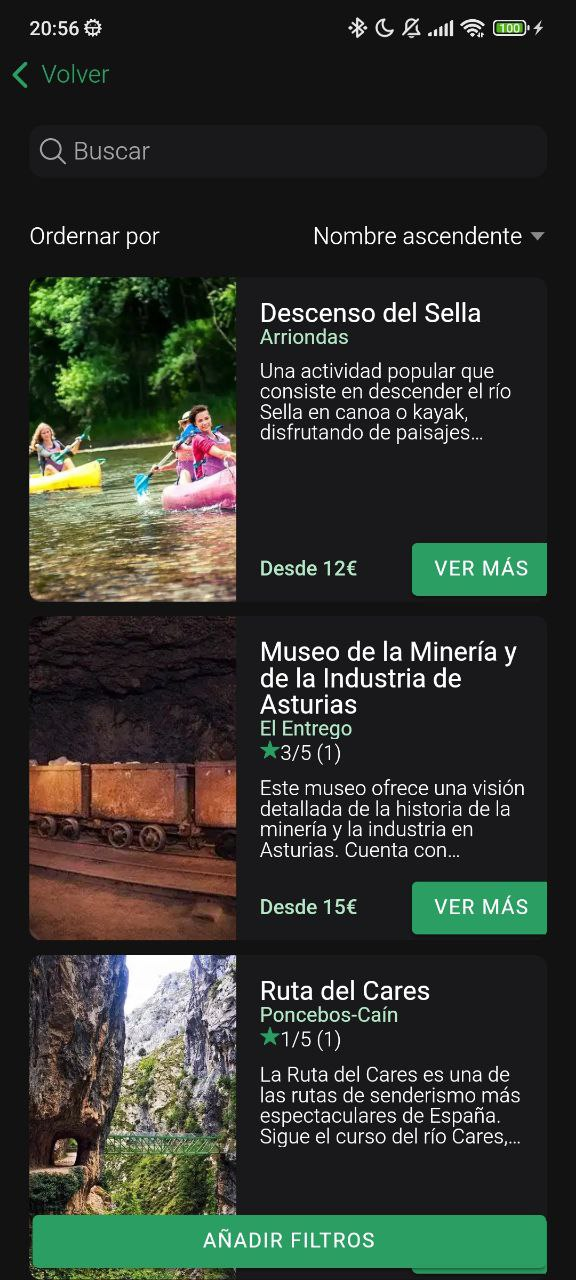
\includegraphics[width=0.18\linewidth]{6-DiseñoDelSistemaDeInformacion/RevisionInterfaces/BuscarActividades/buscar-app.png}
	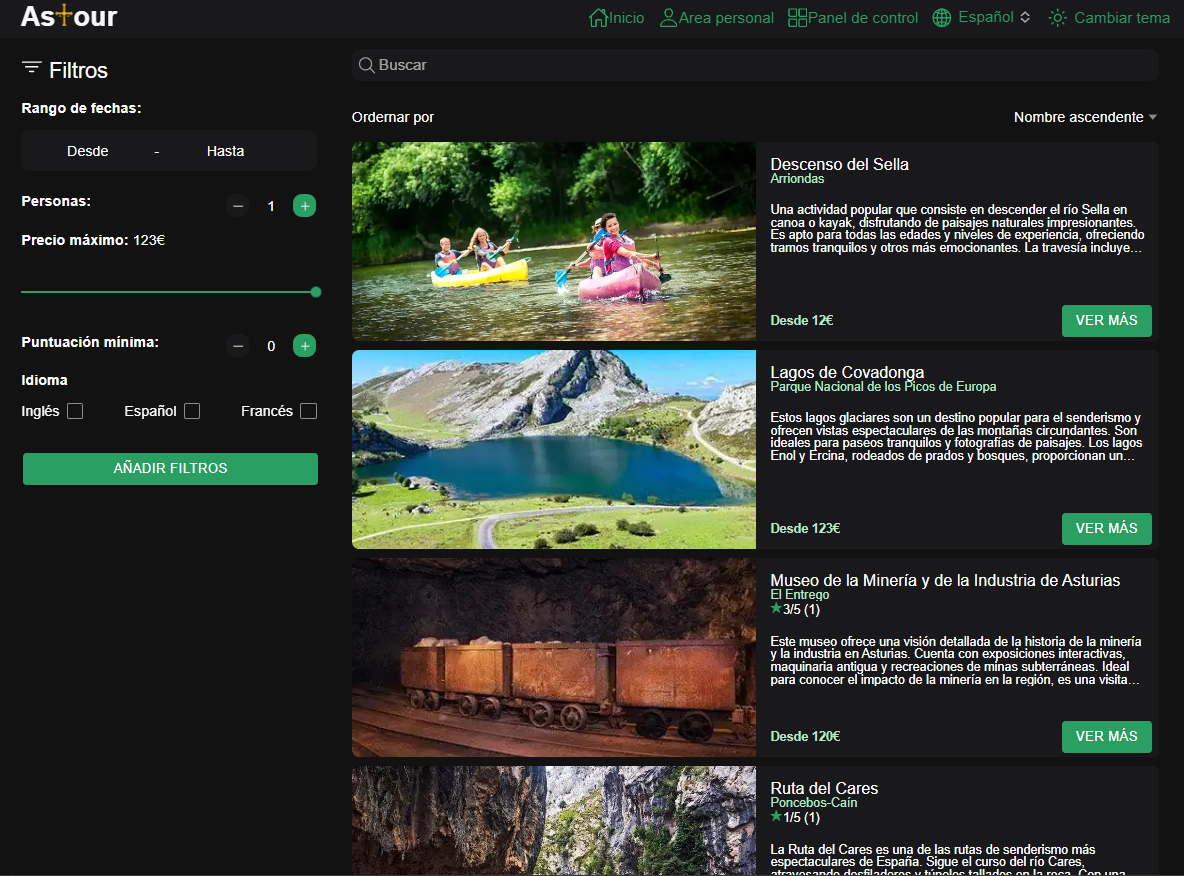
\includegraphics[width=0.5\linewidth]{6-DiseñoDelSistemaDeInformacion/RevisionInterfaces/BuscarActividades/buscar.png}
	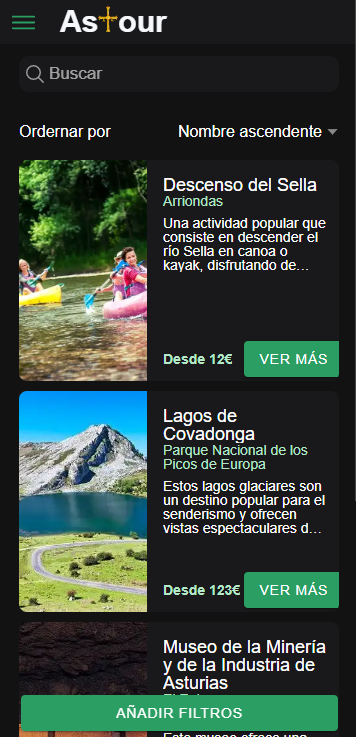
\includegraphics[width=0.18\linewidth]{6-DiseñoDelSistemaDeInformacion/RevisionInterfaces/BuscarActividades/buscar-mobile.png}
	\caption{Buscar Actividades}
\end{figure}

\begin{figure}[H]
	\centering
	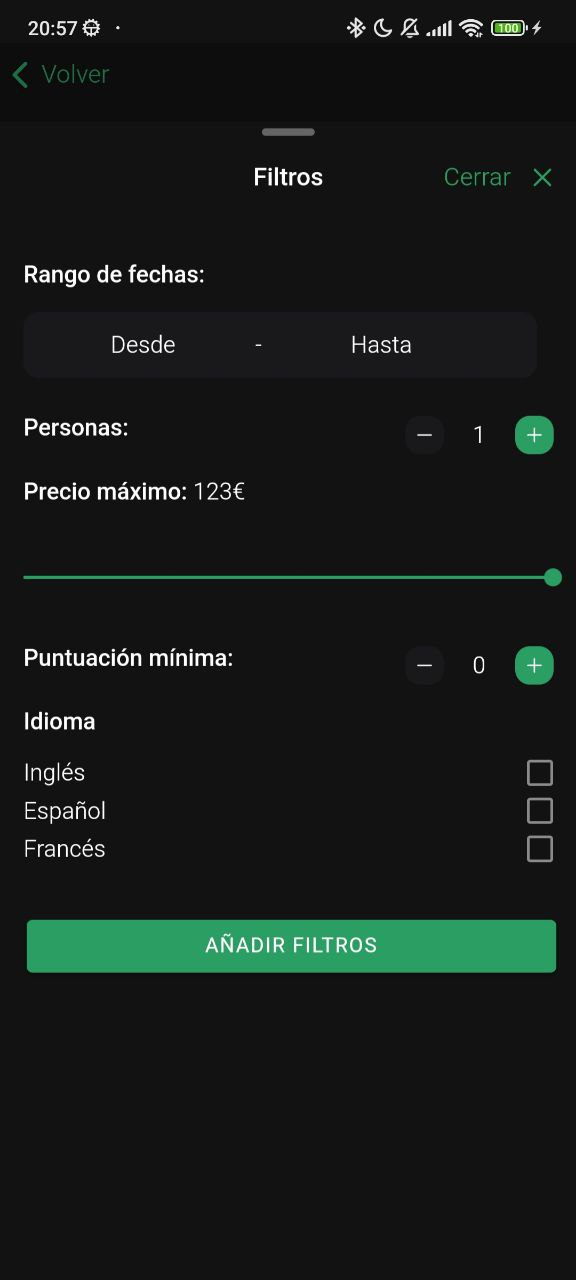
\includegraphics[width=0.18\linewidth]{6-DiseñoDelSistemaDeInformacion/RevisionInterfaces/BuscarActividades/buscar-aplicando-app.png}
	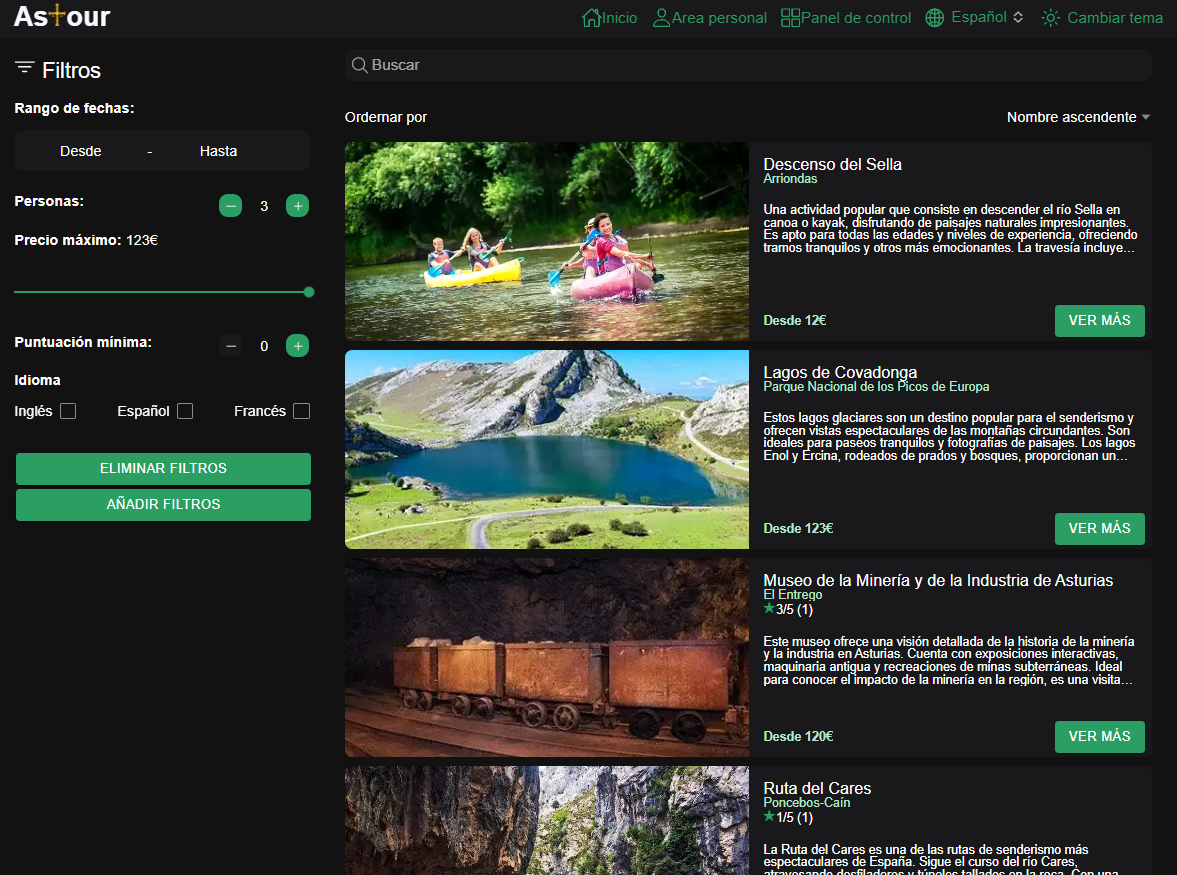
\includegraphics[width=0.5\linewidth]{6-DiseñoDelSistemaDeInformacion/RevisionInterfaces/BuscarActividades/buscar-borrando.png}
	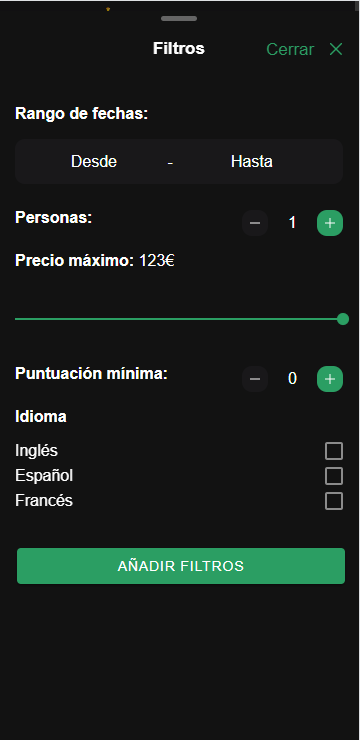
\includegraphics[width=0.18\linewidth]{6-DiseñoDelSistemaDeInformacion/RevisionInterfaces/BuscarActividades/buscar-aplicando-mobile.png}
	\caption{Buscar Actividades - Aplicar Filtros}
\end{figure}

\begin{figure}[H]
	\centering
	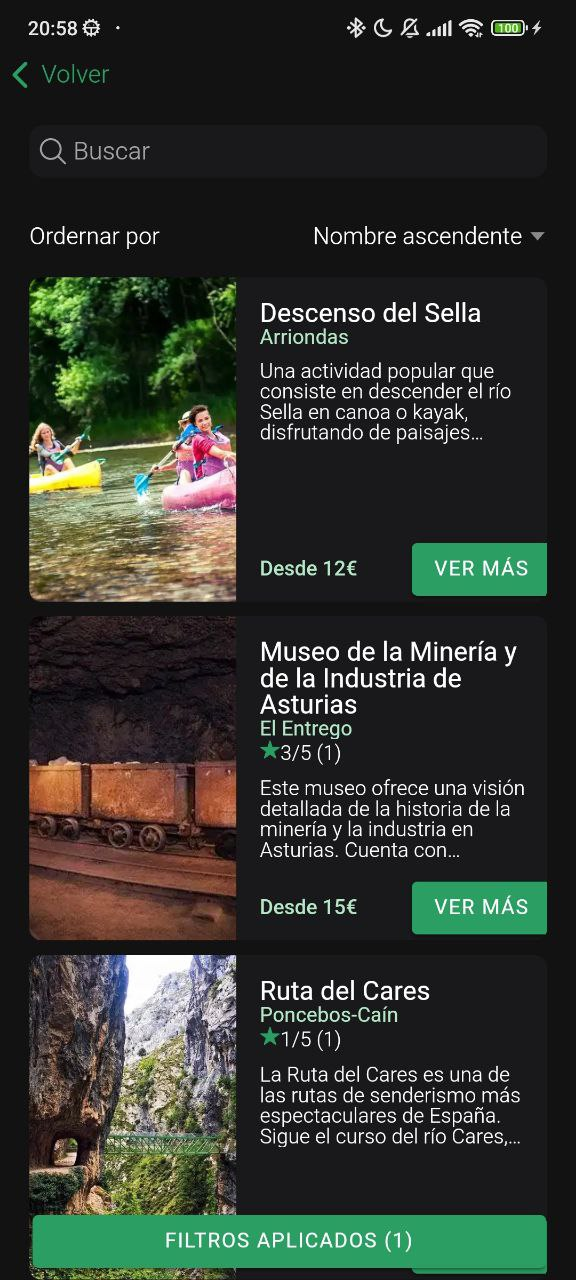
\includegraphics[width=0.18\linewidth]{6-DiseñoDelSistemaDeInformacion/RevisionInterfaces/BuscarActividades/buscar-con-filtros-app.png}
	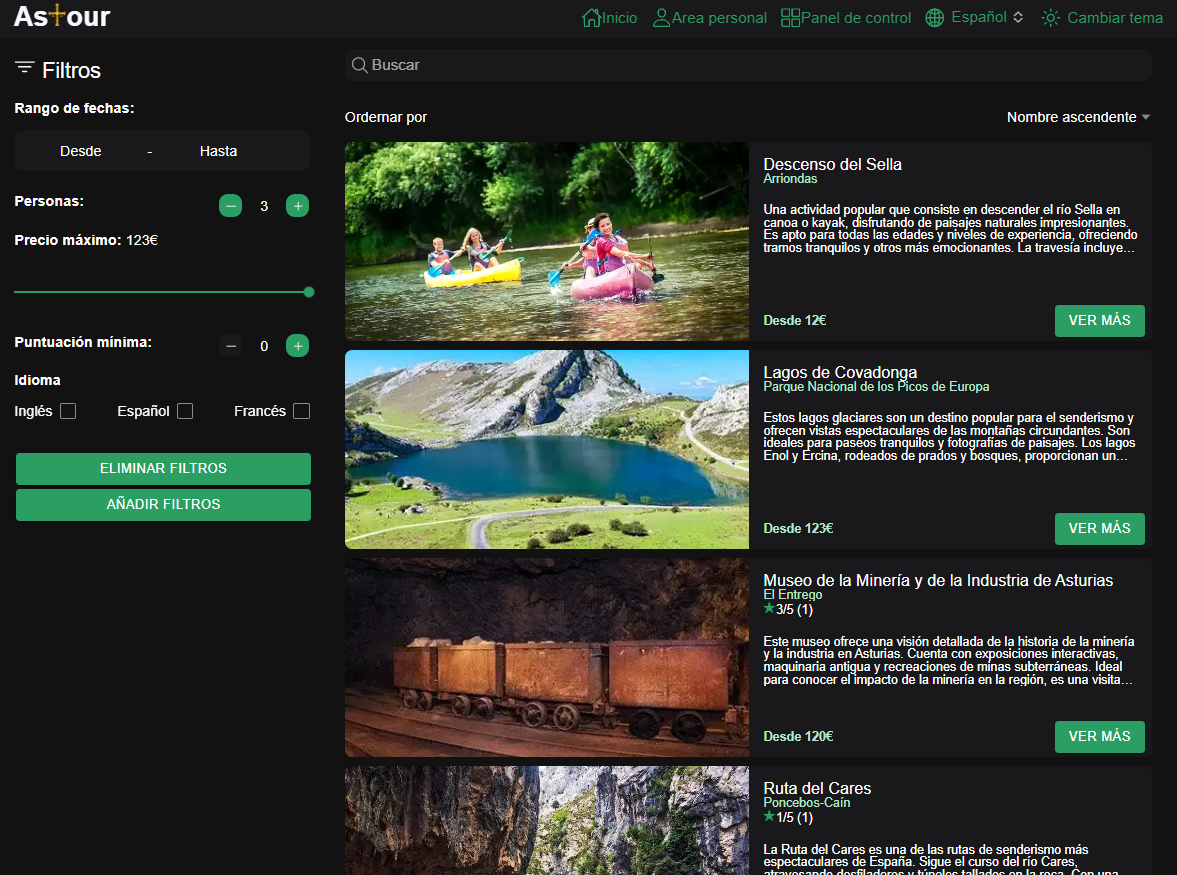
\includegraphics[width=0.5\linewidth]{6-DiseñoDelSistemaDeInformacion/RevisionInterfaces/BuscarActividades/buscar-borrando.png}
	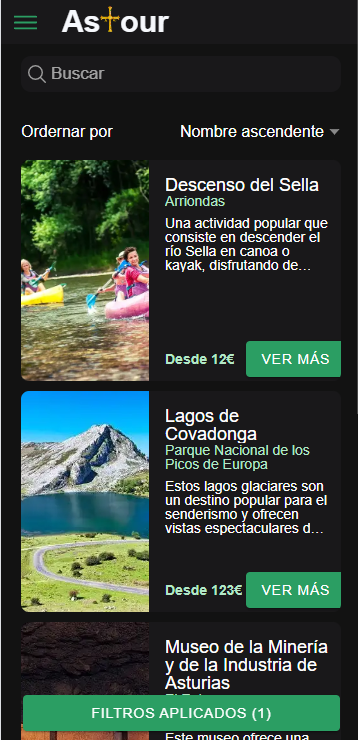
\includegraphics[width=0.18\linewidth]{6-DiseñoDelSistemaDeInformacion/RevisionInterfaces/BuscarActividades/buscar-con-filtros-mobile.png}
	\caption{Buscar Actividades - Con Filtros}
\end{figure}


\begin{figure}[H]
	\centering
	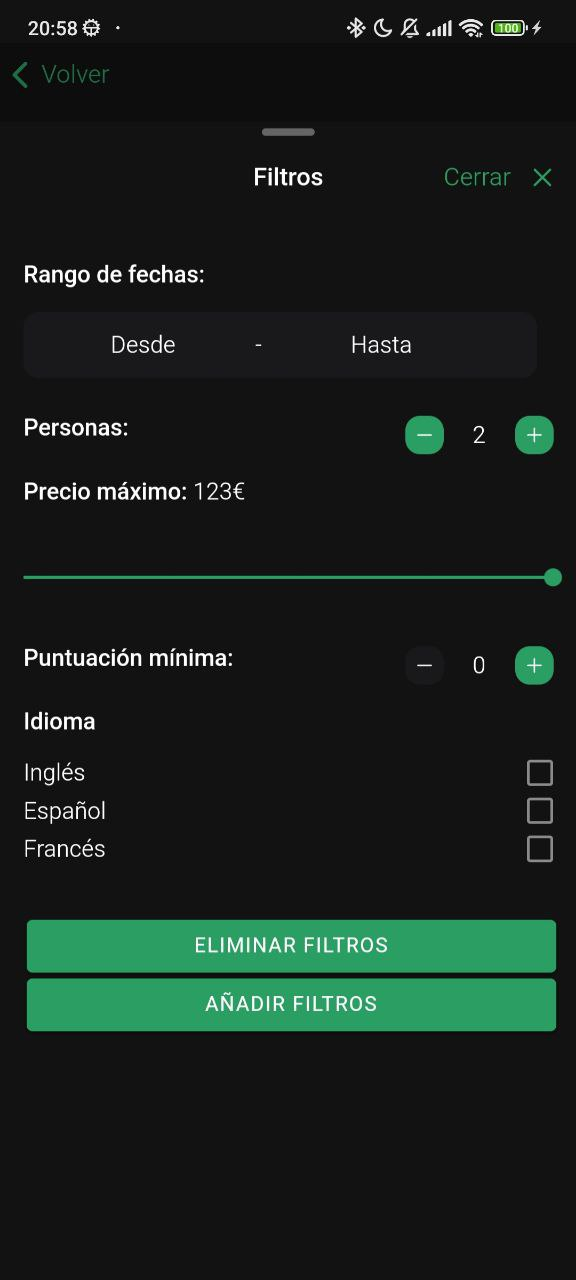
\includegraphics[width=0.18\linewidth]{6-DiseñoDelSistemaDeInformacion/RevisionInterfaces/BuscarActividades/buscar-borrando-app.png}
	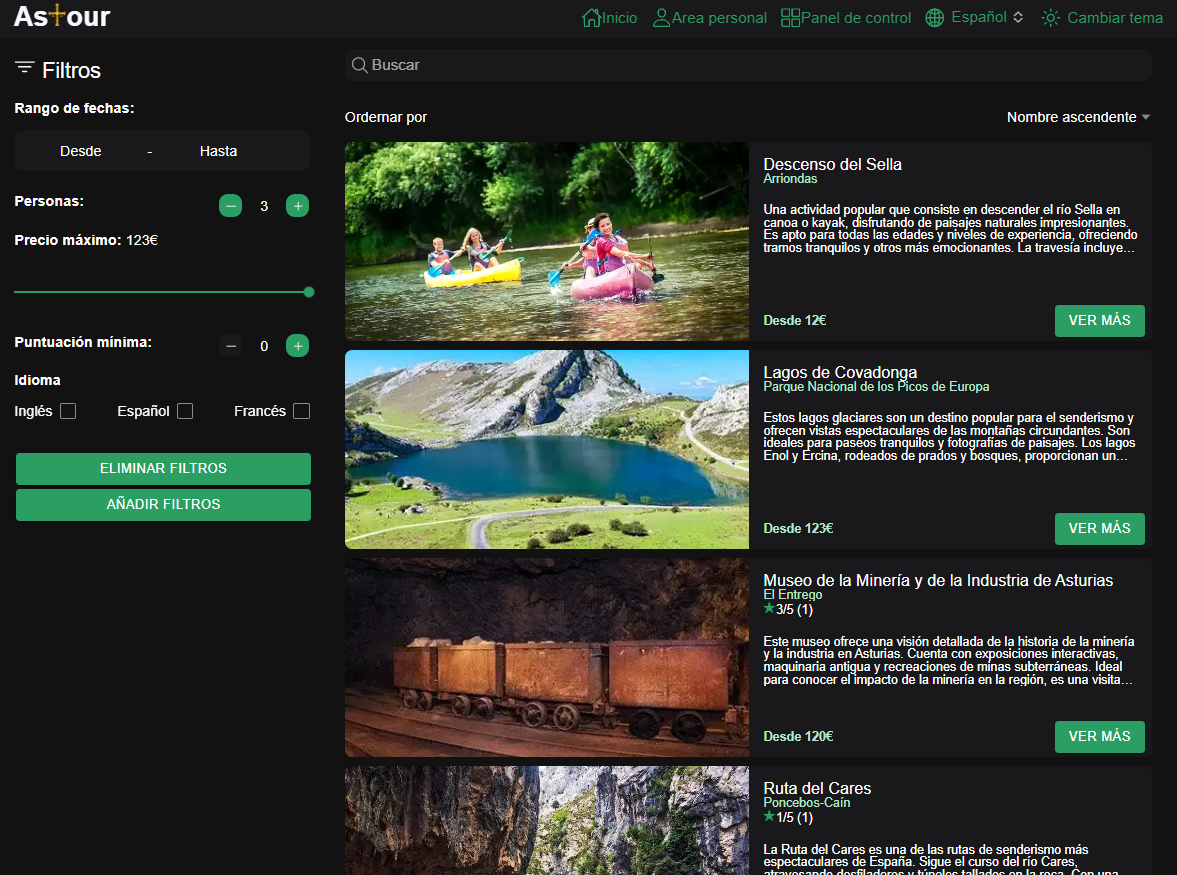
\includegraphics[width=0.5\linewidth]{6-DiseñoDelSistemaDeInformacion/RevisionInterfaces/BuscarActividades/buscar-borrando.png}
	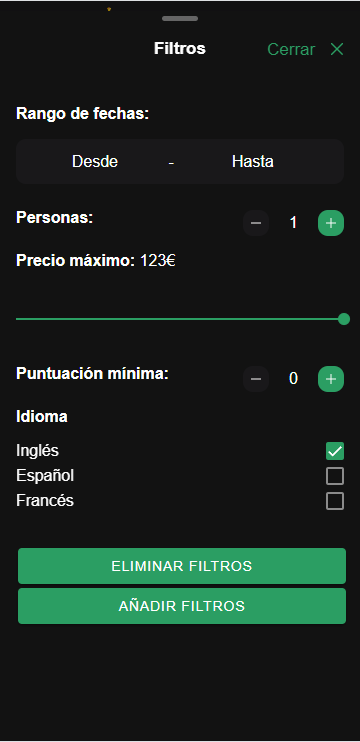
\includegraphics[width=0.18\linewidth]{6-DiseñoDelSistemaDeInformacion/RevisionInterfaces/BuscarActividades/buscar-borrar-mobile.png}
	\caption{Buscar Actividades - Borrar Filtros}
\end{figure}

\subsubsection{Detalles de actividad}
La vista “Detalles de actividad” será aquella vista que se enseñará cuando el usuario quiera ver la información asociada a la actividad. En esta vista el usuario también podrá ver las valoraciones y la disponibilidad en caso de que la actividad tenga eventos con plazas disponibles.
\begin{figure}[H]
	\centering
	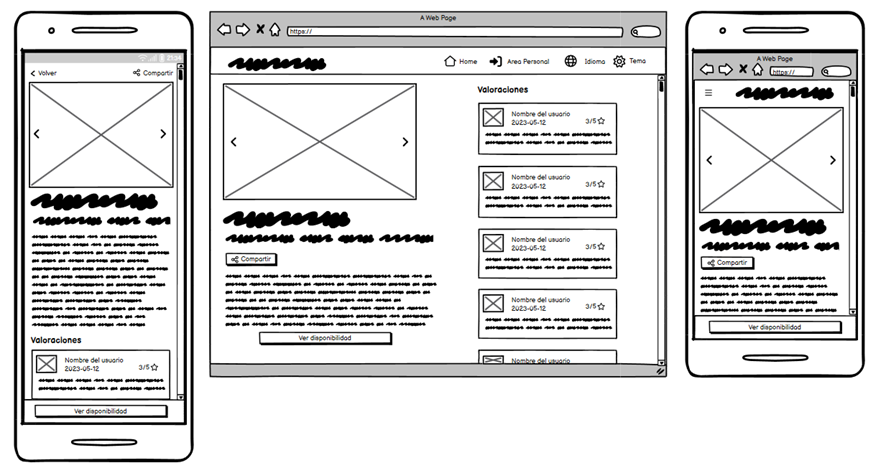
\includegraphics[width=0.8\textwidth]{5-AnalisisDelSistemaDeInformacion/InterfacesDeUsuario/Detalles de actividad/detalles-estandar.png}
	\caption{Detalles de actividad}
\end{figure}

\begin{figure}[H]
	\centering
	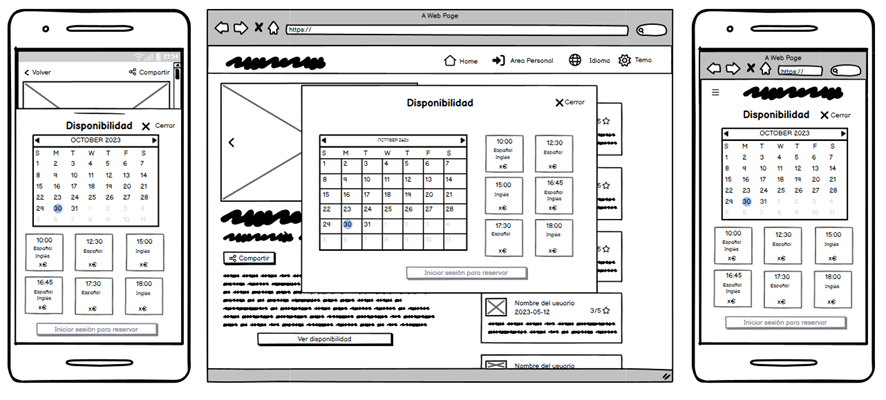
\includegraphics[width=0.8\textwidth]{5-AnalisisDelSistemaDeInformacion/InterfacesDeUsuario/Detalles de actividad/detalles-estandar-disponibilidad.png}
	\caption{Detalles de actividad - Disponibilidad}
\end{figure}
\subsubsection{Realizar reserva}
La vista “Realizar reserva” será aquella vista que se enseñará cuando el usuario quiera empiece el proceso de compra. En esta vista el usuario pasará por distintos pasos donde deberá introducir datos personales y datos bancarios para realizar la reserva.
\begin{figure}[H]
	\centering
	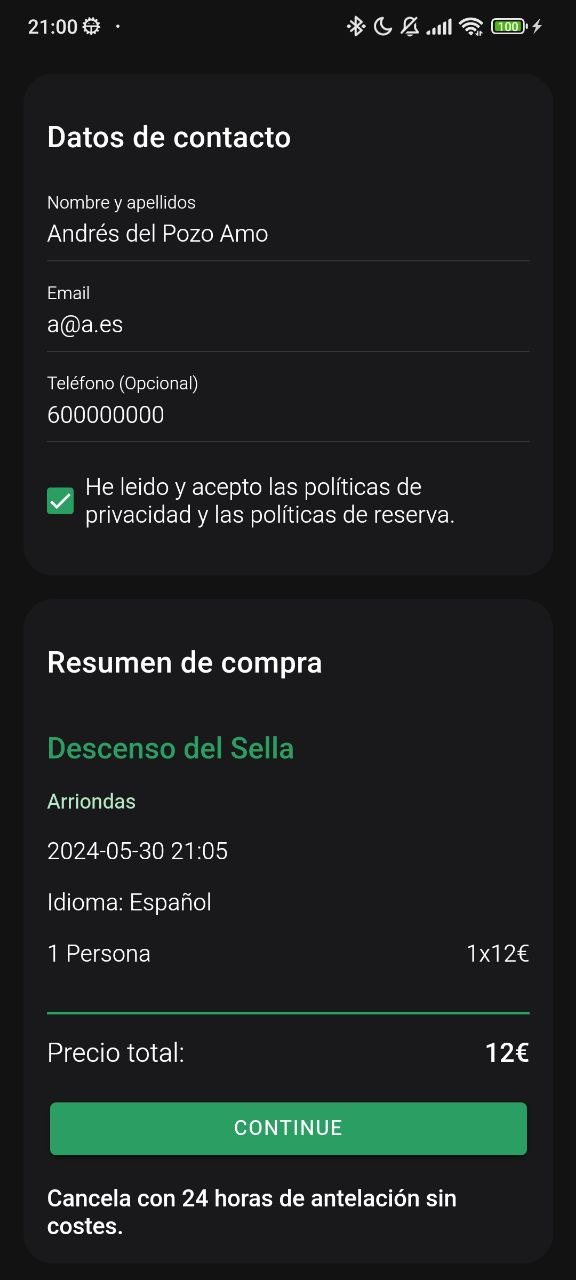
\includegraphics[width=0.18\linewidth]{6-DiseñoDelSistemaDeInformacion/RevisionInterfaces/Reservar/reservar-app.png}
	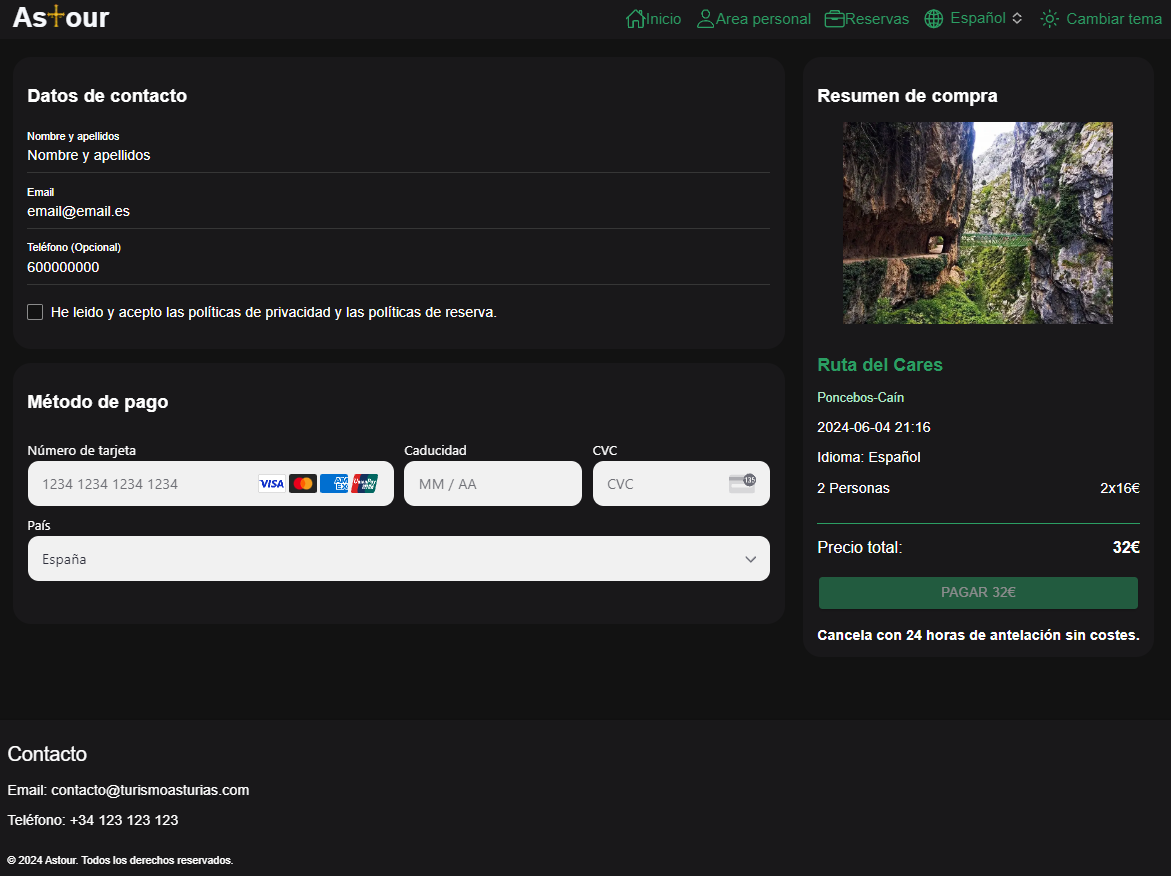
\includegraphics[width=0.5\linewidth]{6-DiseñoDelSistemaDeInformacion/RevisionInterfaces/Reservar/reservar.png}
	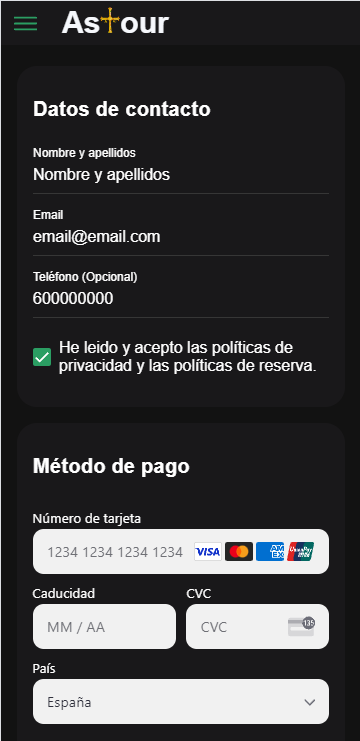
\includegraphics[width=0.18\linewidth]{6-DiseñoDelSistemaDeInformacion/RevisionInterfaces/Reservar/reservar-mobile.png}
	\caption{Realizar reserva - Rellenar datos}
\end{figure}

\begin{figure}[H]
	\centering
	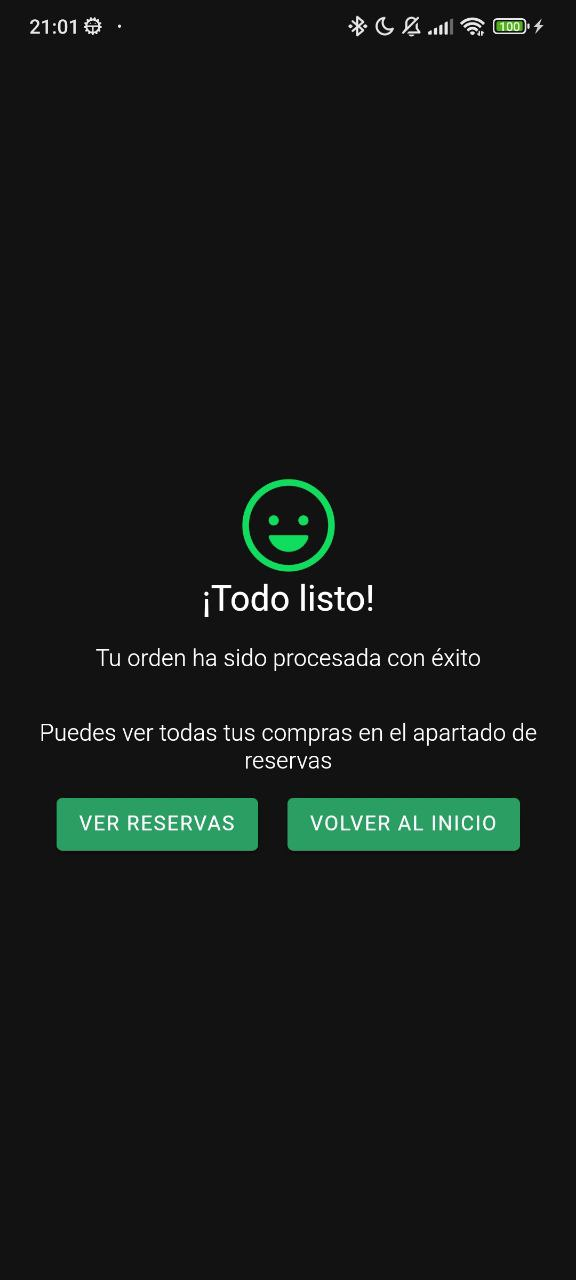
\includegraphics[width=0.18\linewidth]{6-DiseñoDelSistemaDeInformacion/RevisionInterfaces/Reservar/reservar-confirm-app.png}
	\includegraphics[width=0.5\linewidth]{6-DiseñoDelSistemaDeInformacion/RevisionInterfaces/Reservar/reservar-confirm.png}
	\includegraphics[width=0.18\linewidth]{6-DiseñoDelSistemaDeInformacion/RevisionInterfaces/Reservar/reservar-confirm-mobile.png}
	\caption{Realizar reserva - Confirmación}
\end{figure}
\subsubsection{Lista de reservas}
En esta vista “Lista de reservas” el usuario podrá ver todas las reservas realizadas agrupadas por rangos de fechas próximas.
\begin{figure}[H]
	\centering
	\includegraphics[width=0.8\linewidth]{5-AnalisisDelSistemaDeInformacion/InterfacesDeUsuario/Lista de reservas/lista.png}
	\caption{Lista de reservas}
\end{figure}
\subsubsection*{Gestión de reserva}
En esta vista “Gestión de reserva” el usuario podrá ver la información asociada a la reserva, añadir una reseña si ha completado la reserva, así como cancelarla si lo desea.
\begin{figure}[H]
	\centering
	\includegraphics[width=0.18\linewidth]{6-DiseñoDelSistemaDeInformacion/RevisionInterfaces/Detalles de reserva/detalles-app.png}
	\includegraphics[width=0.5\linewidth]{6-DiseñoDelSistemaDeInformacion/RevisionInterfaces/Detalles de reserva/detalles.png}
	\includegraphics[width=0.18\linewidth]{6-DiseñoDelSistemaDeInformacion/RevisionInterfaces/Detalles de reserva/detalles-mobile.png}
	\caption{Gestión de reserva}
\end{figure}
\subsubsection{Perfil}
En esta vista “Perfil” el usuario podrá ver todos sus datos personales, asi como gestionar su cuenta, ya sea para cambiar la contraseña o para cancelar la cuenta.
\begin{figure}[H]
	\centering
	\includegraphics[width=0.8\linewidth]{5-AnalisisDelSistemaDeInformacion/InterfacesDeUsuario/Perfil/perfil-personales.png}
	\caption{Perfil - Datos Personales}
\end{figure}

\begin{figure}[H]
	\centering
	\includegraphics[width=0.8\linewidth]{5-AnalisisDelSistemaDeInformacion/InterfacesDeUsuario/Perfil/perfil-cuenta.png}
	\caption{Perfil - Cuenta}
\end{figure}

\begin{figure}[H]
	\centering
	\includegraphics[width=0.8\linewidth]{5-AnalisisDelSistemaDeInformacion/InterfacesDeUsuario/Perfil/perfil-cambio-personales.png}
	\caption{Perfil - Cambio de Datos Personales}
\end{figure}

\begin{figure}[H]
	\centering
	\includegraphics[width=0.8\linewidth]{5-AnalisisDelSistemaDeInformacion/InterfacesDeUsuario/Perfil/perfil-cambio-contraseña.png}
	\caption{Perfil - Cambio de Contraseña}
\end{figure}
\subsubsection{Dashboard}
En esta vista “Dashboard” el usuario registrado como administrador podrá ver los datos estadísticos de la aplicación, así como gestionar las actividades y los usuarios.
\begin{figure}[H]
	\centering
	\includegraphics[width=0.8\textwidth]{5-AnalisisDelSistemaDeInformacion/InterfacesDeUsuario/Dashboard/panel de control.png}
	\caption{Dashboard - Panel de control}
\end{figure}


En el apartado “Usuarios” de la vista “Dashboard” se muestra una lista de los usuarios registrados en el sistema.
En la tabla se muestra el nombre, correo electrónico, el rol y las reservas realizadas de cada usuario.
Además, se incluye un botón para ver los detalles de cada usuario que nos llevará a la vista “Detalles de usuario” .

\begin{figure}[H]
	\centering
	\includegraphics[width=0.8\textwidth]{5-AnalisisDelSistemaDeInformacion/InterfacesDeUsuario/Dashboard/lista usuarios.png}
	\caption{Dashboard - Lista de usuarios}
\end{figure}

\begin{figure}[H]
	\centering
	\includegraphics[width=0.8\textwidth]{5-AnalisisDelSistemaDeInformacion/InterfacesDeUsuario/Dashboard/lista usuarios edit.png}
	\caption{Dashboard - Editar usuario}
\end{figure}

En el apartado “Actividades” de la vista “Dashboard” se muestra una lista de las actividades registradas en el sistema.
En la tabla se muestra el nombre, fecha de inicio, fecha de fin, lugar, descripción y el estado de cada actividad.
En caso de querer ver los eventos de una actividad, se puede hacer clic en la opción del menú lateral “Mostrar eventos” .

\begin{figure}[H]
	\centering
	\includegraphics[width=0.8\textwidth]{5-AnalisisDelSistemaDeInformacion/InterfacesDeUsuario/Dashboard/lista de actividades.png}
	\caption{Dashboard - Lista de actividades}
\end{figure}

\begin{figure}[H]
	\centering
	\includegraphics[width=0.8\textwidth]{5-AnalisisDelSistemaDeInformacion/InterfacesDeUsuario/Dashboard/lista de actividades edit.png}
	\caption{Dashboard - Lista de actividades}
\end{figure}

\begin{figure}[H]
	\centering
	\includegraphics[width=0.8\textwidth]{5-AnalisisDelSistemaDeInformacion/InterfacesDeUsuario/Dashboard/lista eventos.png}
	\caption{Dashboard - Lista de actividades con eventos}
\end{figure}

\begin{figure}[H]
	\centering
	\includegraphics[width=0.8\textwidth]{5-AnalisisDelSistemaDeInformacion/InterfacesDeUsuario/Dashboard/lista eventos edit.png}
	\caption{Dashboard - Editar evento}
\end{figure}

\subsubsection*{Detalles de usuario}
En la vista “Detalles de usuario” se muestra la información personal de un usuario, así como las reservas realizadas por el mismo.
Además, se incluye un botón para editar los datos del usuario y otro para editar una reserva.

\begin{figure}[H]
	\centering
	\includegraphics[width=0.8\textwidth]{5-AnalisisDelSistemaDeInformacion/InterfacesDeUsuario/Dashboard/detalles usuario.png}
	\caption{Detalles de usuario}
\end{figure}

\begin{figure}[H]
	\centering
	\includegraphics[width=0.8\textwidth]{5-AnalisisDelSistemaDeInformacion/InterfacesDeUsuario/Dashboard/detalles usuario editar datos.png}
	\caption{Detalles de usuario - Editar datos}
\end{figure}

\begin{figure}[H]
	\centering
	\includegraphics[width=0.8\textwidth]{5-AnalisisDelSistemaDeInformacion/InterfacesDeUsuario/Dashboard/detalles usuario editar reserva.png}
	\caption{Detalles de usuario - Editar reserva}
\end{figure}

\subsubsection{Eventos próximos}
En esta vista “Eventos próximos” el usuario registrado como guía podrá ver los eventos que tiene próximamente planificados, así como información de contacto de los turistas que han reservado.
\begin{figure}[H]
	\centering
	\includegraphics[width=0.8\textwidth]{5-AnalisisDelSistemaDeInformacion/InterfacesDeUsuario/EventosProximos/eventos proximos.png}
	\caption{Eventos próximos}
\end{figure}

\begin{figure}[H]
	\centering
	\includegraphics[width=0.8\textwidth]{5-AnalisisDelSistemaDeInformacion/InterfacesDeUsuario/EventosProximos/eventos proximos participantes.png}
	\caption{Eventos próximos - Participantes}
\end{figure}


\section{Diseño físico de la base de datos}
\subsection{Descripción del SGBD Usado}
MongoDB \cite{} ha sido seleccionada como base de datos no relacional por sus características como base de datos NoSQL orientada a documentos. Esta elección se debe a su notable flexibilidad y su capacidad para gestionar grandes volúmenes de datos de manera eficiente, además de ofrecer una escalabilidad horizontal significativa.
\\[1ex]
Para gestionar las comunicaciones con el servidor, se ha implementado el Object-Relational Mapping (ORM) de Mongoose [29]. Este ORM permite tratar la información utilizando esquemas, lo cual proporciona una solución clara y directa. También facilita la administración de datos al ofrecer una amplia interfaz para realizar operaciones CRUD, y su integración con Node.js ha sido clave para considerarlo la opción más adecuada para la gestión de la base de datos.
\\[1ex]
\subsection{Integración del SGBD en nuestro sistema}
Dentro de este sistema, MongoDB se encuentra en el lado del servidor, conectada a la API REST mediante Mongoose como intermediario. La estructura de la base de datos se define utilizando esquemas en Mongoose, los cuales modelan y gestionan las relaciones entre los datos. Los modelos actúan como constructores para facilitar la interacción con la base de datos.
\\[1ex]
\subsection{Colecciones de la base de datos}
A continuación, se describen las distintas colecciones que conforman la base de datos no relacional empleada por el sistema. La estructura de la base de datos en MongoDB está principalmente compuesta por las siguientes colecciones:
\begin{figure}[H]
	\centering
	\includegraphics[width=1\linewidth]{6-DiseñoDelSistemaDeInformacion/SGBD/colecciones.png}
	\caption{Colecciones de la base de datos}
\end{figure}
Para comprender este diagrama, es importante explicar ciertos aspectos relevantes. Los atributos que tienen una “NN” a su derecha indican que no pueden estar vacíos, es decir, son obligatorios. Asimismo, los atributos que aparecen con “[]” representan arrays del tipo especificado y aquellos que muestran “\{\}” indican que son objetos que contienen más atributos en su interior, los cuales se detallan a su derecha.

\section{Especificación técnica del plan de pruebas}
\subsection{Pruebas unitarias}
\subsubsection{activityController.ts}
\begin{small}
	\begin{longtable}[H]{|>{\centering\arraybackslash}m{3cm}|>{\centering\arraybackslash}m{2cm}|>{\centering\arraybackslash}m{3cm}|>{\centering\arraybackslash}m{4cm}|}
		\hline
		\textbf{Función} & \textbf{Tipo de Caso}     & \textbf{Prueba}                                 & \textbf{Resultado Esperado}                                               \\
		\hline
		\endfirsthead
		\multicolumn{4}{c}
		{{\bfseries \tablename\ \thetable{} -- continuación}}                                                                                                                      \\
		\hline
		\textbf{Función} & \textbf{Tipo de Caso}     & \textbf{Prueba}                                 & \textbf{Resultado Esperado}                                               \\
		\hline
		\endhead
		\hline \multicolumn{4}{|r|}{{Continúa en la siguiente página}}                                                                                                             \\ \hline
		\endfoot
		\hline
		\endlastfoot
		\multirow{4}{3cm}{GET /list}
		                 & Filtro de precio inválido & Cuando el filtro de precio es inválido          & Debe responder con un estado 400 y un mensaje de error                    \\
		\cline{2-4}
		                 & Búsqueda válida           & Cuando la búsqueda es válida                    & Debe responder con un estado 200 y las actividades                        \\
		\cline{2-4}
		                 & Error por defecto         & Cuando el servicio lanza un error por defecto   & Debe responder con un estado 500 y un mensaje de error genérico           \\
		\cline{2-4}
		                 & Error personalizado       & Cuando el servicio lanza un error personalizado & Debe responder con el estado y mensaje del error personalizado            \\
		\hline

		\multirow{3}{3cm}{GET /:id}
		                 & ID válido                 & Cuando el ID es válido                          & Debe responder con un estado 200 y la actividad                           \\
		\cline{2-4}
		                 & Error por defecto         & Cuando el servicio lanza un error por defecto   & Debe responder con un estado 500 y un mensaje de error genérico           \\
		\cline{2-4}
		                 & Error personalizado       & Cuando el servicio lanza un error personalizado & Debe responder con el estado y mensaje del error personalizado            \\
		\hline

		\multirow{3}{3cm}{GET /:id/events}
		                 & ID válido                 & Cuando el ID es válido                          & Debe responder con un estado 200 y los eventos                            \\
		\cline{2-4}
		                 & Error por defecto         & Cuando el servicio lanza un error por defecto   & Debe responder con un estado 500 y un mensaje de error genérico           \\
		\cline{2-4}
		                 & Error personalizado       & Cuando el servicio lanza un error personalizado & Debe responder con el estado y mensaje del error personalizado            \\
		\hline

		\multirow{3}{3cm}{GET /event/:id}
		                 & ID válido                 & Cuando el ID es válido                          & Debe responder con un estado 200 y la actividad correspondiente al evento \\
		\cline{2-4}
		                 & Error por defecto         & Cuando el servicio lanza un error por defecto   & Debe responder con un estado 500 y un mensaje de error genérico           \\
		\cline{2-4}
		                 & Error personalizado       & Cuando el servicio lanza un error personalizado & Debe responder con el estado y mensaje del error personalizado            \\
		\hline

		\multirow{3}{3cm}{GET /:id/reviews}
		                 & ID válido                 & Cuando el ID es válido                          & Debe responder con un estado 200 y las reseñas                            \\
		\cline{2-4}
		                 & Error por defecto         & Cuando el servicio lanza un error por defecto   & Debe responder con un estado 500 y un mensaje de error genérico           \\
		\cline{2-4}
		                 & Error personalizado       & Cuando el servicio lanza un error personalizado & Debe responder con el estado y mensaje del error personalizado            \\
		\hline
		\caption{Pruebas unitarias de activityController.ts}
	\end{longtable}
\end{small}

\subsubsection{activityService.ts}
\begin{small}
	\begin{longtable}[H]{|>{\centering\arraybackslash}m{3cm}|>{\centering\arraybackslash}m{2cm}|>{\centering\arraybackslash}m{3cm}|>{\centering\arraybackslash}m{4cm}|}
		\hline
		\textbf{Función}                    & \textbf{Tipo de Caso}       & \textbf{Prueba}                                             & \textbf{Resultado Esperado}                                           \\
		\hline
		\endfirsthead
		\multicolumn{4}{c}
		{{\bfseries \tablename\ \thetable{} -- continuación}}                                                                                                                                                   \\
		\hline
		\textbf{Función}                    & \textbf{Tipo de Caso}       & \textbf{Prueba}                                             & \textbf{Resultado Esperado}                                           \\
		\hline
		\endhead
		\hline \multicolumn{4}{|r|}{{Continúa en la siguiente página}}                                                                                                                                          \\ \hline
		\endfoot
		\hline
		\endlastfoot
		\multirow{2}{4cm}{getAllActivities} & \multirow{2}{3cm}{Positivo} & Cuando se encuentran actividades y hay filtros de precio    & Debe responder con actividades                                        \\
		\cline{3-4}
		                                    &                             & Cuando se encuentran actividades y no hay filtros de precio & Debe responder con actividades                                        \\
		\hline
		\multirow{4}{4cm}{getOneActivity}   & \multirow{1}{3cm}{Positivo} & Cuando se encuentra la actividad                            & Debe responder con una actividad                                      \\
		\cline{2-4}
		                                    & \multirow{3}{3cm}{Negativo} & Cuando el ID de la actividad no es válido                   & Debe lanzar un error indicando que el identificador no es válido      \\
		\cline{3-4}
		                                    &                             & Cuando no se encuentra la actividad                         & Debe lanzar un error indicando que la actividad no fue encontrada     \\
		\cline{3-4}
		                                    &                             & Cuando hay un error en el servidor                          & Debe lanzar un error indicando un problema en el servidor             \\
		\hline
		\multirow{4}{4cm}{getEvents}        & \multirow{2}{3cm}{Positivo} & Cuando hay eventos para la actividad                        & Debe responder con los eventos                                        \\
		\cline{3-4}
		                                    &                             & Cuando no hay eventos para la actividad                     & Debe lanzar un error indicando que no hay eventos para esta actividad \\
		\cline{2-4}
		                                    & \multirow{2}{3cm}{Negativo} & Cuando la actividad no existe                               & Debe lanzar un error indicando que la actividad no fue encontrada     \\
		\cline{3-4}
		                                    &                             & Cuando el ID de la actividad no es válido                   & Debe lanzar un error indicando que el ID no es válido                 \\
		\hline
		\caption{Pruebas unitarias de activityService.ts}
	\end{longtable}
\end{small}

\subsubsection{adminActivityController.ts}
\begin{small}
	\begin{longtable}[H]{|>{\centering\arraybackslash}m{3cm}|>{\centering\arraybackslash}m{2cm}|>{\centering\arraybackslash}m{3cm}|>{\centering\arraybackslash}m{4cm}|}
		\hline
		\textbf{Función}                              & \textbf{Tipo de Caso}       & \textbf{Prueba}                                             & \textbf{Resultado Esperado}                                             \\
		\hline
		\endfirsthead
		\multicolumn{4}{c}
		{{\bfseries \tablename\ \thetable{} -- continuación}}                                                                                                                                                               \\
		\hline
		\textbf{Función}                              & \textbf{Tipo de Caso}       & \textbf{Prueba}                                             & \textbf{Resultado Esperado}                                             \\
		\hline
		\endhead
		\hline \multicolumn{4}{|r|}{{Continúa en la siguiente página}}                                                                                                                                                      \\ \hline
		\endfoot
		\hline
		\endlastfoot
		\multirow{4}{4cm}{POST /}                     & \multirow{2}{3cm}{Positivo} & Cuando los datos de la nueva actividad son correctos        & Responder con un código de estado 200 y un mensaje de éxito             \\
		\cline{3-4}
		                                              &                             & Cuando los datos de la nueva actividad están ausentes       & Responder con un código de estado 400 y un mensaje de error             \\
		\cline{2-4}
		                                              & \multirow{2}{3cm}{Negativo} & Cuando el adminActivityService lanza un error por defecto   & Responder con un código de estado 500 y un mensaje de error de servidor \\
		\cline{3-4}
		                                              &                             & Cuando el adminActivityService lanza un error personalizado & Responder con el código de estado del error personalizado y su mensaje  \\
		\hline
		\multirow{4}{4cm}{PUT /:id}                   & \multirow{2}{3cm}{Positivo} & Cuando los cambios son correctos                            & Responder con un código de estado 200 y un mensaje de éxito             \\
		\cline{3-4}
		                                              &                             & Cuando los cambios están ausentes                           & Responder con un código de estado 400 y un mensaje de error             \\
		\cline{2-4}
		                                              & \multirow{2}{3cm}{Negativo} & Cuando el adminActivityService lanza un error por defecto   & Responder con un código de estado 500 y un mensaje de error de servidor \\
		\cline{3-4}
		                                              &                             & Cuando el adminActivityService lanza un error personalizado & Responder con el código de estado del error personalizado y su mensaje  \\
		\hline
		\multirow{4}{4cm}{DELETE /:id}                & \multirow{2}{3cm}{Positivo} & Cuando la actividad es eliminada                            & Responder con un código de estado 200 y un mensaje de éxito             \\
		\cline{2-4}
		                                              & \multirow{2}{3cm}{Negativo} & Cuando el adminActivityService lanza un error por defecto   & Responder con un código de estado 500 y un mensaje de error de servidor \\
		\cline{3-4}
		                                              &                             & Cuando el adminActivityService lanza un error personalizado & Responder con el código de estado del error personalizado y su mensaje  \\
		\hline
		\multirow{7}{4cm}{POST /:activityId/events}   & \multirow{2}{3cm}{Positivo} & Cuando se añade un solo evento                              & Responder con un código de estado 200 y un mensaje de éxito             \\
		\cline{3-4}
		                                              &                             & Cuando se añade un solo evento con repeatInfo days          & Responder con un código de estado 200 y un mensaje de éxito             \\
		\cline{2-4}
		                                              & \multirow{5}{3cm}{Negativo} & Cuando el adminActivityService lanza un error por defecto   & Responder con un código de estado 500 y un mensaje de error de servidor \\
		\cline{3-4}
		                                              &                             & Cuando el adminActivityService lanza un error personalizado & Responder con el código de estado del error personalizado y su mensaje  \\
		\cline{3-4}
		                                              &                             & Cuando faltan datos del evento a añadir                     & Responder con un código de estado 400 y un mensaje de error             \\
		\cline{3-4}
		                                              &                             & Cuando falta una fecha o repeatInfo                         & Responder con un código de estado 400 y un mensaje de error             \\
		\cline{3-4}
		                                              &                             & Cuando falta un rango de fechas válido para el evento       & Responder con un código de estado 400 y un mensaje de error             \\
		\hline
		\multirow{3}{4cm}{DELETE /:activityId/review} & \multirow{1}{3cm}{Positivo} & Cuando el comentario es eliminado                           & Responder con un código de estado 200 y un mensaje de éxito             \\
		\cline{2-4}
		                                              & \multirow{2}{3cm}{Negativo} & Cuando el adminActivityService lanza un error por defecto   & Responder con un código de estado 500 y un mensaje de error de servidor \\
		\cline{3-4}
		                                              &                             & Cuando el adminActivityService lanza un error personalizado & Responder con el código de estado del error personalizado y su mensaje  \\
		\hline
		\multirow{3}{4cm}{GET /event/list}            & \multirow{1}{3cm}{Positivo} & Cuando se recuperan los eventos                             & Responder con un código de estado 200 y una lista de eventos            \\
		\cline{2-4}
		                                              & \multirow{2}{3cm}{Negativo} & Cuando el adminActivityService lanza un error por defecto   & Responder con un código de estado 500 y un mensaje de error de servidor \\
		\cline{3-4}
		                                              &                             & Cuando el adminActivityService lanza un error personalizado & Responder con el código de estado del error personalizado y su mensaje  \\
		\hline
		\multirow{3}{4cm}{GET /list}                  & \multirow{1}{3cm}{Positivo} & Cuando se recuperan las actividades                         & Responder con un código de estado 200 y una lista de actividades        \\
		\cline{2-4}
		                                              & \multirow{2}{3cm}{Negativo} & Cuando el adminActivityService lanza un error por defecto   & Responder con un código de estado 500 y un mensaje de error de servidor \\
		\cline{3-4}
		                                              &                             & Cuando el adminActivityService lanza un error personalizado & Responder con el código de estado del error personalizado y su mensaje  \\
		\hline
		\caption{Pruebas unitarias de adminActivityController.ts}
	\end{longtable}
\end{small}

\subsubsection{adminActivityService.ts}
\begin{small}
	\begin{longtable}[H]{|>{\centering\arraybackslash}m{3cm}|>{\centering\arraybackslash}m{2cm}|>{\centering\arraybackslash}m{3cm}|>{\centering\arraybackslash}m{4cm}|}
		\hline
		\textbf{Función}                    & \textbf{Tipo de Caso}       & \textbf{Prueba}                           & \textbf{Resultado Esperado}                                       \\
		\hline
		\endfirsthead
		\multicolumn{4}{c}
		{{\bfseries \tablename\ \thetable{} -- continuación}}                                                                                                                             \\
		\hline
		\textbf{Función}                    & \textbf{Tipo de Caso}       & \textbf{Prueba}                           & \textbf{Resultado Esperado}                                       \\
		\hline
		\endhead
		\hline \multicolumn{4}{|r|}{{Continúa en la siguiente página}}                                                                                                                    \\ \hline
		\endfoot
		\hline
		\endlastfoot
		\multirow{3}{4cm}{Add new activity} & Positivo                    & Cuando la actividad es añadida            & Debe responder con la actividad                                   \\
		\cline{2-4}
		                                    & \multirow{2}{3cm}{Negativo} & Cuando la actividad no es válida          & Debe responder con el error                                       \\
		\cline{3-4}
		                                    &                             & Cuando hay un error                       & Debe responder con el error                                       \\
		\hline
		\multirow{4}{4cm}{Edit activity}    & Positivo                    & Cuando la actividad es editada            & Debe responder con la actividad                                   \\
		\cline{2-4}
		                                    & \multirow{3}{3cm}{Negativo} & Cuando el ID de la actividad no es válido & Debe lanzar un error indicando que el ID no es válido             \\
		\cline{3-4}
		                                    &                             & Cuando la actividad no es encontrada      & Debe lanzar un error indicando que la actividad no fue encontrada \\
		\cline{3-4}
		                                    &                             & Cuando hay un error                       & Debe lanzar un error indicando un problema en el servidor         \\
		\hline
		\multirow{4}{4cm}{Delete activity}  & Positivo                    & Cuando la actividad es eliminada          & Debe responder con la actividad                                   \\
		\cline{2-4}
		                                    & \multirow{3}{3cm}{Negativo} & Cuando el ID de la actividad no es válido & Debe lanzar un error indicando que el ID no es válido             \\
		\cline{3-4}
		                                    &                             & Cuando la actividad no es encontrada      & Debe lanzar un error indicando que la actividad no fue encontrada \\
		\cline{3-4}
		                                    &                             & Cuando hay un error                       & Debe lanzar un error indicando un problema en el servidor         \\
		\hline
		\multirow{5}{4cm}{Add events}       & Positivo                    & Cuando los eventos son añadidos           & Debe responder con la actividad                                   \\
		\cline{2-4}
		                                    & \multirow{4}{3cm}{Negativo} & Cuando el ID de la actividad no es válido & Debe lanzar un error indicando que el ID no es válido             \\
		\cline{3-4}
		                                    &                             & Cuando la actividad no es encontrada      & Debe lanzar un error indicando que la actividad no fue encontrada \\
		\cline{3-4}
		                                    &                             & Cuando el guía no es encontrado           & Debe lanzar un error indicando que el guía no fue encontrado      \\
		\cline{3-4}
		                                    &                             & Cuando hay un error                       & Debe lanzar un error indicando un problema en el servidor         \\
		\hline
		\multirow{5}{4cm}{Delete review}    & Positivo                    & Cuando el comentario es eliminado         & Debe responder con la actividad                                   \\
		\cline{2-4}
		                                    & \multirow{4}{3cm}{Negativo} & Cuando el ID de la actividad no es válido & Debe lanzar un error indicando que el ID no es válido             \\
		\cline{3-4}
		                                    &                             & Cuando el ID de la review no es válido    & Debe lanzar un error indicando que el ID no es válido             \\
		\cline{3-4}
		                                    &                             & Cuando la actividad no es encontrada      & Debe lanzar un error indicando que la actividad no fue encontrada \\
		\cline{3-4}
		                                    &                             & Cuando hay un error                       & Debe lanzar un error indicando un problema en el servidor         \\
		\hline
		\caption{Pruebas unitarias de adminActivityService.ts}
	\end{longtable}
\end{small}
\subsubsection{adminUserController.ts}
\begin{small}
	\begin{longtable}[H]{|>{\centering\arraybackslash}m{3cm}|>{\centering\arraybackslash}m{2cm}|>{\centering\arraybackslash}m{3cm}|>{\centering\arraybackslash}m{4cm}|}
		\hline
		\textbf{Función}                                 & \textbf{Tipo de Caso}       & \textbf{Prueba}                                               & \textbf{Resultado Esperado}                                             \\
		\hline
		\endfirsthead
		\multicolumn{4}{c}
		{{\bfseries \tablename\ \thetable{} -- continuación}}                                                                                                                                                                    \\
		\hline
		\textbf{Función}                                 & \textbf{Tipo de Caso}       & \textbf{Prueba}                                               & \textbf{Resultado Esperado}                                             \\
		\hline
		\endhead
		\hline \multicolumn{4}{|r|}{{Continúa en la siguiente página}}                                                                                                                                                           \\ \hline
		\endfoot
		\hline
		\endlastfoot
		\multirow{7}{4cm}{POST /}                        & Positivo                    & Cuando los datos del nuevo usuario son correctos              & Responder con un código de estado 200 y un mensaje de éxito             \\
		\cline{2-4}
		                                                 & \multirow{6}{3cm}{Negativo} & Cuando faltan los datos del nuevo usuario                     & Responder con un código de estado 400 y un mensaje de error             \\
		\cline{3-4}
		                                                 &                             & Cuando los datos del nuevo usuario están incompletos          & Responder con un código de estado 400 y un mensaje de error             \\
		\cline{3-4}
		                                                 &                             & Cuando los datos del nuevo usuario están vacíos               & Responder con un código de estado 400 y un mensaje de error             \\
		\cline{3-4}
		                                                 &                             & Cuando los datos del nuevo usuario son nulos                  & Responder con un código de estado 400 y un mensaje de error             \\
		\cline{3-4}
		                                                 &                             & Cuando los datos del nuevo usuario son indefinidos            & Responder con un código de estado 400 y un mensaje de error             \\
		\cline{3-4}
		                                                 &                             & Cuando el adminUserService lanza un error personalizado       & Responder con el código de estado del error personalizado y su mensaje  \\
		\hline
		\multirow{3}{4cm}{GET /list}                     & Positivo                    & Cuando el adminUserService devuelve una lista de usuarios     & Responder con un código de estado 200 y la lista de usuarios            \\
		\cline{2-4}
		                                                 & \multirow{2}{3cm}{Negativo} & Cuando el adminUserService lanza un error por defecto         & Responder con un código de estado 500 y un mensaje de error de servidor \\
		\cline{3-4}
		                                                 &                             & Cuando el adminUserService lanza un error personalizado       & Responder con el código de estado del error personalizado y su mensaje  \\
		\hline
		\multirow{3}{4cm}{GET /:id}                      & Positivo                    & Cuando el adminUserService devuelve un usuario                & Responder con un código de estado 200 y el usuario                      \\
		\cline{2-4}
		                                                 & \multirow{2}{3cm}{Negativo} & Cuando el adminUserService lanza un error por defecto         & Responder con un código de estado 500 y un mensaje de error de servidor \\
		\cline{3-4}
		                                                 &                             & Cuando el adminUserService lanza un error personalizado       & Responder con el código de estado del error personalizado y su mensaje  \\
		\hline
		\multirow{3}{4cm}{DELETE /:id}                   & Positivo                    & Cuando el adminUserService elimina un usuario                 & Responder con un código de estado 200 y un mensaje de éxito             \\
		\cline{2-4}
		                                                 & \multirow{2}{3cm}{Negativo} & Cuando el adminUserService lanza un error por defecto         & Responder con un código de estado 500 y un mensaje de error de servidor \\
		\cline{3-4}
		                                                 &                             & Cuando el adminUserService lanza un error personalizado       & Responder con el código de estado del error personalizado y su mensaje  \\
		\hline
		\multirow{3}{4cm}{PUT /:id}                      & Positivo                    & Cuando el adminUserService edita un usuario                   & Responder con un código de estado 200 y un mensaje de éxito             \\
		\cline{2-4}
		                                                 & \multirow{2}{3cm}{Negativo} & Cuando el adminUserService lanza un error por defecto         & Responder con un código de estado 500 y un mensaje de error de servidor \\
		\cline{3-4}
		                                                 &                             & Cuando el adminUserService lanza un error personalizado       & Responder con el código de estado del error personalizado y su mensaje  \\
		\hline
		\multirow{3}{4cm}{GET /:userId/reservation/list} & Positivo                    & Cuando el adminUserService devuelve una lista de reservas     & Responder con un código de estado 200 y la lista de reservas            \\
		\cline{2-4}
		                                                 & \multirow{2}{3cm}{Negativo} & Cuando el adminUserService lanza un error por defecto         & Responder con un código de estado 500 y un mensaje de error de servidor \\
		\cline{3-4}
		                                                 &                             & Cuando el adminUserService lanza un error personalizado       & Responder con el código de estado del error personalizado y su mensaje  \\
		\hline
		\multirow{3}{4cm}{GET /workers}                  & Positivo                    & Cuando el adminUserService devuelve una lista de trabajadores & Responder con un código de estado 200 y la lista de trabajadores        \\
		\cline{2-4}
		                                                 & \multirow{2}{3cm}{Negativo} & Cuando el adminUserService lanza un error por defecto         & Responder con un código de estado 500 y un mensaje de error de servidor \\
		\cline{3-4}
		                                                 &                             & Cuando el adminUserService lanza un error personalizado       & Responder con el código de estado del error personalizado y su mensaje  \\
		\hline
		\multirow{3}{4cm}{GET /reservation/list}         & Positivo                    & Cuando el adminUserService devuelve una lista de reservas     & Responder con un código de estado 200 y la lista de reservas            \\
		\cline{2-4}
		                                                 & \multirow{2}{3cm}{Negativo} & Cuando el adminUserService lanza un error por defecto         & Responder con un código de estado 500 y un mensaje de error de servidor \\
		\cline{3-4}
		                                                 &                             & Cuando el adminUserService lanza un error personalizado       & Responder con el código de estado del error personalizado y su mensaje  \\
		\hline
		\caption{Pruebas unitarias de adminUserController.ts}
	\end{longtable}
\end{small}

\subsubsection{adminUserService.ts}
\begin{small}
	\begin{longtable}[H]{|>{\centering\arraybackslash}m{3cm}|>{\centering\arraybackslash}m{2cm}|>{\centering\arraybackslash}m{3cm}|>{\centering\arraybackslash}m{4cm}|}
		\hline
		\textbf{Función}                 & \textbf{Tipo de Caso}       & \textbf{Prueba}                                       & \textbf{Resultado Esperado}                                                \\
		\hline
		\endfirsthead
		\multicolumn{4}{c}
		{{\bfseries \tablename\ \thetable{} -- continuación}}                                                                                                                                               \\
		\hline
		\textbf{Función}                 & \textbf{Tipo de Caso}       & \textbf{Prueba}                                       & \textbf{Resultado Esperado}                                                \\
		\hline
		\endhead
		\hline \multicolumn{4}{|r|}{{Continúa en la siguiente página}}                                                                                                                                      \\ \hline
		\endfoot
		\hline
		\endlastfoot
		\multirow{5}{4cm}{Add user}      & Positivo                    & Cuando el usuario no está registrado                  & Debe retornar el usuario                                                   \\
		\cline{2-4}
		                                 & \multirow{4}{3cm}{Negativo} & Cuando el usuario está registrado                     & Debe lanzar un error indicando que el email ya está registrado             \\
		\cline{3-4}
		                                 &                             & Cuando el rol no es correcto                          & Debe lanzar un error indicando que el rol es incorrecto                    \\
		\cline{3-4}
		                                 &                             & Cuando hay un error en la búsqueda                    & Debe lanzar un error indicando un problema en el servidor                  \\
		\cline{3-4}
		                                 &                             & Cuando hay un error al guardar                        & Debe lanzar un error indicando un problema en el servidor                  \\
		\hline
		\multirow{4}{4cm}{Get all users} & Positivo                    & Cuando hay usuarios                                   & Debe retornar los usuarios                                                 \\
		\cline{2-4}
		                                 & \multirow{3}{3cm}{Negativo} & Cuando no hay usuarios                                & Debe lanzar un error indicando que no se encontraron usuarios              \\
		\cline{3-4}
		                                 &                             & Cuando hay un error en la búsqueda                    & Debe lanzar un error indicando un problema en el servidor                  \\
		\cline{3-4}
		                                 &                             & Cuando hay un error en las opciones de consulta       & Debe lanzar un error indicando un problema en el servidor                  \\
		\hline
		\multirow{4}{4cm}{Get one user}  & Positivo                    & Cuando hay un usuario                                 & Debe retornar el usuario                                                   \\
		\cline{2-4}
		                                 & \multirow{3}{3cm}{Negativo} & Cuando no hay un usuario                              & Debe lanzar un error indicando que no se encontraron los datos del usuario \\
		\cline{3-4}
		                                 &                             & Cuando el id no es válido                             & Debe lanzar un error indicando que el id no es válido                      \\
		\cline{3-4}
		                                 &                             & Cuando hay un error en la búsqueda                    & Debe lanzar un error indicando un problema en el servidor                  \\
		\hline
		\multirow{4}{4cm}{Delete user}   & Positivo                    & Cuando el usuario es eliminado                        & No debe lanzar un error                                                    \\
		\cline{2-4}
		                                 & \multirow{3}{3cm}{Negativo} & Cuando el usuario no es encontrado                    & Debe lanzar un error indicando que el usuario no fue encontrado            \\
		\cline{3-4}
		                                 &                             & Cuando el id no es válido                             & Debe lanzar un error indicando que el id no es válido                      \\
		\cline{3-4}
		                                 &                             & Cuando hay un error en la búsqueda                    & Debe lanzar un error indicando un problema en el servidor                  \\
		\hline
		\multirow{4}{4cm}{Edit user}     & Positivo                    & Cuando el usuario es editado                          & No debe lanzar un error                                                    \\
		\cline{2-4}
		                                 & \multirow{3}{3cm}{Negativo} & Cuando el usuario no es encontrado                    & Debe lanzar un error indicando que el usuario no fue encontrado            \\
		\cline{3-4}
		                                 &                             & Cuando el id no es válido                             & Debe lanzar un error indicando que el id no es válido                      \\
		\cline{3-4}
		                                 &                             & Cuando hay un error en la búsqueda                    & Debe lanzar un error indicando un problema en el servidor                  \\
		\hline
		\multirow{5}{4cm}{Get workers}   & \multirow{5}{3cm}{Positivo} & Cuando hay trabajadores sin eventos asignados         & Debe retornar los trabajadores                                             \\
		\cline{3-4}
		                                 &                             & Cuando hay trabajadores con algunos eventos asignados & Debe retornar los trabajadores                                             \\
		\cline{3-4}
		                                 &                             & Cuando no hay trabajadores en repeatType none         & Debe retornar una lista vacía                                              \\
		\cline{3-4}
		                                 &                             & Cuando no hay trabajadores en repeatType days         & Debe retornar una lista vacía                                              \\
		\cline{3-4}
		                                 &                             & Cuando no hay trabajadores en repeatType range        & Debe retornar una lista vacía                                              \\
		\hline
		\multirow{2}{4cm}{Get workers}   & \multirow{2}{3cm}{Negativo} & Cuando hay un error en la búsqueda                    & Debe lanzar un error indicando un problema en el servidor                  \\
		\cline{3-4}
		                                 &                             & Cuando hay un error en las opciones de consulta       & Debe lanzar un error indicando un problema en el servidor                  \\
		\hline
		\caption{Pruebas unitarias de adminUserService.ts}
	\end{longtable}
\end{small}

\subsubsection{authController.ts}
\begin{small}
	\begin{longtable}[H]{|>{\centering\arraybackslash}m{3cm}|>{\centering\arraybackslash}m{2cm}|>{\centering\arraybackslash}m{3cm}|>{\centering\arraybackslash}m{4cm}|}
		\hline
		\textbf{Función}                  & \textbf{Tipo de Caso}       & \textbf{Prueba}                                          & \textbf{Resultado Esperado}                                             \\
		\hline
		\endfirsthead
		\multicolumn{4}{c}
		{{\bfseries \tablename\ \thetable{} -- continuación}}                                                                                                                                                \\
		\hline
		\textbf{Función}                  & \textbf{Tipo de Caso}       & \textbf{Prueba}                                          & \textbf{Resultado Esperado}                                             \\
		\hline
		\endhead
		\hline \multicolumn{4}{|r|}{{Continúa en la siguiente página}}                                                                                                                                       \\ \hline
		\endfoot
		\hline
		\endlastfoot
		\multirow{5}{4cm}{POST /login}    & Positivo                    & Cuando el usuario inicia sesión con credenciales válidas & Responder con un código de estado 200 y el cuerpo correcto              \\
		\cline{2-4}
		                                  & \multirow{4}{3cm}{Negativo} & Cuando falta el email                                    & Responder con un código de estado 400 y un mensaje de error             \\
		\cline{3-4}
		                                  &                             & Cuando falta la contraseña                               & Responder con un código de estado 400 y un mensaje de error             \\
		\cline{3-4}
		                                  &                             & Cuando el authService lanza un error por defecto         & Responder con un código de estado 500 y un mensaje de error de servidor \\
		\cline{3-4}
		                                  &                             & Cuando el authService lanza un error personalizado       & Responder con el código de estado del error personalizado y su mensaje  \\
		\hline
		\multirow{6}{4cm}{POST /register} & Positivo                    & Cuando el usuario se registra con credenciales válidas   & Responder con un código de estado 200 y un mensaje de éxito             \\
		\cline{2-4}
		                                  &                             & Cuando el usuario se registra con campos opcionales      & Responder con un código de estado 200 y un mensaje de éxito             \\
		\cline{2-4}
		                                  & \multirow{4}{3cm}{Negativo} & Cuando falta el nombre                                   & Responder con un código de estado 400 y un mensaje de error             \\
		\cline{3-4}
		                                  &                             & Cuando falta el email                                    & Responder con un código de estado 400 y un mensaje de error             \\
		\cline{3-4}
		                                  &                             & Cuando falta la contraseña                               & Responder con un código de estado 400 y un mensaje de error             \\
		\cline{3-4}
		                                  &                             & Cuando el authService lanza un error por defecto         & Responder con un código de estado 500 y un mensaje de error de servidor \\
		\cline{2-4}
		                                  & \multirow{1}{3cm}{Negativo} & Cuando el authService lanza un error personalizado       & Responder con el código de estado del error personalizado y su mensaje  \\
		\hline
		\caption{Pruebas unitarias de authController.ts}
	\end{longtable}
\end{small}

\subsubsection{authService.ts}
\begin{small}
	\begin{longtable}[H]{|>{\centering\arraybackslash}m{3cm}|>{\centering\arraybackslash}m{2cm}|>{\centering\arraybackslash}m{3cm}|>{\centering\arraybackslash}m{4cm}|}
		\hline
		\textbf{Función}            & \textbf{Tipo de Caso}       & \textbf{Prueba}                     & \textbf{Resultado Esperado}                                         \\
		\hline
		\endfirsthead
		\multicolumn{4}{c}
		{{\bfseries \tablename\ \thetable{} -- continuación}}                                                                                                                 \\
		\hline
		\textbf{Función}            & \textbf{Tipo de Caso}       & \textbf{Prueba}                     & \textbf{Resultado Esperado}                                         \\
		\hline
		\endhead
		\hline \multicolumn{4}{|r|}{{Continúa en la siguiente página}}                                                                                                        \\ \hline
		\endfoot
		\hline
		\endlastfoot
		\multirow{3}{4cm}{Login}    & Positivo                    & Cuando las credenciales son válidas & Debe responder con un usuario y un token                            \\
		\cline{2-4}
		                            & \multirow{2}{3cm}{Negativo} & Cuando el email no está registrado  & Debe lanzar un error indicando que las credenciales son incorrectas \\
		\cline{3-4}
		                            &                             & Cuando la contraseña es incorrecta  & Debe lanzar un error indicando que las credenciales son incorrectas \\
		\hline
		\multirow{5}{4cm}{Register} & Positivo                    & Cuando el email no está registrado  & Debe guardar el usuario                                             \\
		\cline{2-4}
		                            & \multirow{4}{3cm}{Negativo} & Cuando el email ya está registrado  & Debe lanzar un error indicando que el email ya está registrado      \\
		\cline{3-4}
		                            &                             & Cuando el usuario no es válido      & Debe lanzar un error indicando un problema en el servidor           \\
		\cline{3-4}
		                            &                             & Cuando hay un error                 & Debe lanzar un error indicando un problema en el servidor           \\
		\cline{3-4}
		                            &                             & Cuando hay un error al guardar      & Debe lanzar un error indicando un problema en el servidor           \\
		\hline
		\caption{Pruebas unitarias de authService.ts}
	\end{longtable}
\end{small}

\subsubsection{dashboardController.ts}
\begin{small}
	\begin{longtable}[H]{|>{\centering\arraybackslash}m{3cm}|>{\centering\arraybackslash}m{2cm}|>{\centering\arraybackslash}m{3cm}|>{\centering\arraybackslash}m{4cm}|}
		\hline
		\textbf{Función} & \textbf{Tipo de Caso} & \textbf{Prueba}                                             & \textbf{Resultado Esperado}                                    \\
		\hline
		\endfirsthead
		\multicolumn{4}{c}
		{{\bfseries \tablename\ \thetable{} -- continuación}}                                                                                                                   \\
		\hline
		\textbf{Función} & \textbf{Tipo de Caso} & \textbf{Prueba}                                             & \textbf{Resultado Esperado}                                    \\
		\hline
		\endhead
		\hline \multicolumn{4}{|r|}{{Continúa en la siguiente página}}                                                                                                          \\ \hline
		\endfoot
		\hline
		\endlastfoot
		\multirow{3}{3cm}{GET /totalReservations}
		                 & Llamada exitosa       & Cuando se llama a getTotalReservations                      & Debe responder con un estado 200 y el total de reservas        \\
		\cline{2-4}
		                 & Error por defecto     & Cuando getTotalReservations lanza un error por defecto      & Debe responder con un estado 500 y un mensaje de error         \\
		\cline{2-4}
		                 & Error personalizado   & Cuando getTotalReservations lanza un error personalizado    & Debe responder con el estado y mensaje del error personalizado \\
		\hline

		\multirow{3}{3cm}{GET /totalIncome}
		                 & Llamada exitosa       & Cuando se llama a getTotalIncome                            & Debe responder con un estado 200 y el total de ingresos        \\
		\cline{2-4}
		                 & Error por defecto     & Cuando getTotalIncome lanza un error por defecto            & Debe responder con un estado 500 y un mensaje de error         \\
		\cline{2-4}
		                 & Error personalizado   & Cuando getTotalIncome lanza un error personalizado          & Debe responder con el estado y mensaje del error personalizado \\
		\hline

		\multirow{3}{3cm}{GET /occupation}
		                 & Llamada exitosa       & Cuando se llama a getOccupation                             & Debe responder con un estado 200 y la ocupación                \\
		\cline{2-4}
		                 & Error por defecto     & Cuando getOccupation lanza un error por defecto             & Debe responder con un estado 500 y un mensaje de error         \\
		\cline{2-4}
		                 & Error personalizado   & Cuando getOccupation lanza un error personalizado           & Debe responder con el estado y mensaje del error personalizado \\
		\hline

		\multirow{3}{3cm}{GET /totalUsers}
		                 & Llamada exitosa       & Cuando se llama a getTotalUsers                             & Debe responder con un estado 200 y el total de usuarios        \\
		\cline{2-4}
		                 & Error por defecto     & Cuando getTotalUsers lanza un error por defecto             & Debe responder con un estado 500 y un mensaje de error         \\
		\cline{2-4}
		                 & Error personalizado   & Cuando getTotalUsers lanza un error personalizado           & Debe responder con el estado y mensaje del error personalizado \\
		\hline

		\multirow{3}{3cm}{GET /cancelationRate}
		                 & Llamada exitosa       & Cuando se llama a getCancelationRate                        & Debe responder con un estado 200 y la tasa de cancelación      \\
		\cline{2-4}
		                 & Error por defecto     & Cuando getCancelationRate lanza un error por defecto        & Debe responder con un estado 500 y un mensaje de error         \\
		\cline{2-4}
		                 & Error personalizado   & Cuando getCancelationRate lanza un error personalizado      & Debe responder con el estado y mensaje del error personalizado \\
		\hline

		\multirow{3}{3cm}{GET /categoryReservations}
		                 & Llamada exitosa       & Cuando se llama a getCategoryReservations                   & Debe responder con un estado 200 y las reservas por categoría  \\
		\cline{2-4}
		                 & Error por defecto     & Cuando getCategoryReservations lanza un error por defecto   & Debe responder con un estado 500 y un mensaje de error         \\
		\cline{2-4}
		                 & Error personalizado   & Cuando getCategoryReservations lanza un error personalizado & Debe responder con el estado y mensaje del error personalizado \\
		\hline

		\multirow{3}{3cm}{GET /resume}
		                 & Llamada exitosa       & Cuando se llama a getResume                                 & Debe responder con un estado 200 y el resumen                  \\
		\cline{2-4}
		                 & Error por defecto     & Cuando getResume lanza un error por defecto                 & Debe responder con un estado 500 y un mensaje de error         \\
		\cline{2-4}
		                 & Error personalizado   & Cuando getResume lanza un error personalizado               & Debe responder con el estado y mensaje del error personalizado \\
		\hline

		\multirow{3}{3cm}{GET /reservations}
		                 & Llamada exitosa       & Cuando se llama a getReservations                           & Debe responder con un estado 200 y las reservas                \\
		\cline{2-4}
		                 & Error por defecto     & Cuando getReservations lanza un error por defecto           & Debe responder con un estado 500 y un mensaje de error         \\
		\cline{2-4}
		                 & Error personalizado   & Cuando getReservations lanza un error personalizado         & Debe responder con el estado y mensaje del error personalizado \\
		\hline
		\caption{Pruebas unitarias de dashboardController.ts}
	\end{longtable}
\end{small}

\subsubsection{dashboardService.ts}
\begin{small}
	\begin{longtable}[H]{|>{\centering\arraybackslash}m{3cm}|>{\centering\arraybackslash}m{2cm}|>{\centering\arraybackslash}m{3cm}|>{\centering\arraybackslash}m{4cm}|}
		\hline
		\textbf{Función} & \textbf{Tipo de Caso}       & \textbf{Prueba}                          & \textbf{Resultado Esperado}                                              \\
		\hline
		\endfirsthead
		\multicolumn{4}{c}
		{{\bfseries \tablename\ \thetable{} -- continuación}}                                                                                                                \\
		\hline
		\textbf{Función} & \textbf{Tipo de Caso}       & \textbf{Prueba}                          & \textbf{Resultado Esperado}                                              \\
		\hline
		\endhead
		\hline \multicolumn{4}{|r|}{{Continúa en la siguiente página}}                                                                                                       \\ \hline
		\endfoot
		\hline
		\endlastfoot
		\multirow{3}{3cm}{Get total reservations}
		                 & Reservaciones totales       & Retornar el total de reservaciones       & Debe retornar 5                                                          \\
		\cline{2-4}
		                 & Error por defecto           & Cuando se lanza un error por defecto     & Debe lanzar un error con el mensaje 'Error'                              \\
		\cline{2-4}
		                 & Error personalizado         & Cuando se lanza un error personalizado   & Debe lanzar un error con el estado y mensaje del error personalizado     \\
		\hline

		\multirow{3}{3cm}{Get total income}
		                 & Ingreso total               & Retornar el ingreso total                & Debe retornar 5                                                          \\
		\cline{2-4}
		                 & Error por defecto           & Cuando se lanza un error por defecto     & Debe lanzar un error con el mensaje 'Error'                              \\
		\cline{2-4}
		                 & Error personalizado         & Cuando se lanza un error personalizado   & Debe lanzar un error con el estado y mensaje del error personalizado     \\
		\hline

		\multirow{3}{3cm}{Get occupation}
		                 & Ocupación                   & Retornar la ocupación                    & Debe retornar la tasa de ocupación y los puntos de ocupación             \\
		\cline{2-4}
		                 & Error por defecto           & Cuando se lanza un error por defecto     & Debe lanzar un error con el mensaje 'Error'                              \\
		\cline{2-4}
		                 & Error personalizado         & Cuando se lanza un error personalizado   & Debe lanzar un error con el estado y mensaje del error personalizado     \\
		\hline

		\multirow{1}{3cm}{Get total users}
		                 & Usuarios totales            & Retornar el total de usuarios            & Debe retornar 5                                                          \\
		\hline

		\multirow{3}{3cm}{Get cancelation rate}
		                 & Tasa de cancelación         & Retornar la tasa de cancelación          & Debe retornar la tasa de cancelación y las cancelaciones por día del mes \\
		\cline{2-4}
		                 & Error por defecto           & Cuando se lanza un error por defecto     & Debe lanzar un error con el mensaje 'Error'                              \\
		\cline{2-4}
		                 & Error personalizado         & Cuando se lanza un error personalizado   & Debe lanzar un error con el estado y mensaje del error personalizado     \\
		\hline

		\multirow{3}{3cm}{Get category reservations}
		                 & Reservaciones por categoría & Retornar las reservaciones por categoría & Debe retornar las reservaciones por categoría                            \\
		\cline{2-4}
		                 & Error por defecto           & Cuando se lanza un error por defecto     & Debe lanzar un error con el mensaje 'Error'                              \\
		\cline{2-4}
		                 & Error personalizado         & Cuando se lanza un error personalizado   & Debe lanzar un error con el estado y mensaje del error personalizado     \\
		\hline

		\multirow{3}{3cm}{Get reservations}
		                 & Reservaciones               & Retornar las reservaciones               & Debe retornar las reservaciones con información de la actividad          \\
		\cline{2-4}
		                 & Error por defecto           & Cuando se lanza un error por defecto     & Debe lanzar un error con el mensaje 'Error'                              \\
		\cline{2-4}
		                 & Error personalizado         & Cuando se lanza un error personalizado   & Debe lanzar un error con el estado y mensaje del error personalizado     \\
		\hline
		\caption{Pruebas unitarias de dashboardService.ts}
	\end{longtable}
\end{small}

\subsubsection{eventController.ts}
\begin{small}
	\begin{longtable}[H]{|>{\centering\arraybackslash}m{3cm}|>{\centering\arraybackslash}m{2cm}|>{\centering\arraybackslash}m{3cm}|>{\centering\arraybackslash}m{4cm}|}
		\hline
		\textbf{Función}                          & \textbf{Tipo de Caso}       & \textbf{Prueba}                                     & \textbf{Resultado Esperado}                                 \\
		\hline
		\endfirsthead
		\multicolumn{4}{c}
		{{\bfseries \tablename\ \thetable{} -- continuación}}                                                                                                                                       \\
		\hline
		\textbf{Función}                          & \textbf{Tipo de Caso}       & \textbf{Prueba}                                     & \textbf{Resultado Esperado}                                 \\
		\hline
		\endhead
		\hline \multicolumn{4}{|r|}{{Continúa en la siguiente página}}                                                                                                                              \\ \hline
		\endfoot
		\hline
		\endlastfoot
		\multirow{3}{4cm}{GET /:id}               & Positivo                    & Cuando el evento existe                             & Debe retornar el evento                                     \\
		\cline{2-4}
		                                          & \multirow{2}{3cm}{Negativo} & Cuando el eventService lanza un error por defecto   & Debe retornar un código de estado 500 y un mensaje de error \\
		\cline{3-4}
		                                          &                             & Cuando el eventService lanza un error personalizado & Debe retornar un código de estado 404 y un mensaje de error \\
		\hline
		\multirow{3}{4cm}{GET /:id/participants}  & Positivo                    & Cuando los participantes existen                    & Debe retornar los participantes                             \\
		\cline{2-4}
		                                          & \multirow{2}{3cm}{Negativo} & Cuando el eventService lanza un error por defecto   & Debe retornar un código de estado 500 y un mensaje de error \\
		\cline{3-4}
		                                          &                             & Cuando el eventService lanza un error personalizado & Debe retornar un código de estado 404 y un mensaje de error \\
		\hline
		\multirow{3}{4cm}{GET /list/:id}          & Positivo                    & Cuando los eventos existen                          & Debe retornar los eventos                                   \\
		\cline{2-4}
		                                          & \multirow{2}{3cm}{Negativo} & Cuando el eventService lanza un error por defecto   & Debe retornar un código de estado 500 y un mensaje de error \\
		\cline{3-4}
		                                          &                             & Cuando el eventService lanza un error personalizado & Debe retornar un código de estado 404 y un mensaje de error \\
		\hline
		\multirow{3}{4cm}{DELETE /:id/recurrence} & Positivo                    & Cuando los eventos son eliminados                   & Debe retornar un código de estado 200 y un mensaje de éxito \\
		\cline{2-4}
		                                          & \multirow{2}{3cm}{Negativo} & Cuando el eventService lanza un error por defecto   & Debe retornar un código de estado 500 y un mensaje de error \\
		\cline{3-4}
		                                          &                             & Cuando el eventService lanza un error personalizado & Debe retornar un código de estado 404 y un mensaje de error \\
		\hline
		\caption{Pruebas unitarias de eventController.ts}
	\end{longtable}
\end{small}

\subsubsection{eventService.ts}
\begin{small}
	\begin{longtable}[H]{|>{\centering\arraybackslash}m{3cm}|>{\centering\arraybackslash}m{2cm}|>{\centering\arraybackslash}m{3cm}|>{\centering\arraybackslash}m{4cm}|}
		\hline
		\textbf{Función}                     & \textbf{Tipo de Caso}       & \textbf{Prueba}                          & \textbf{Resultado Esperado}                                    \\
		\hline
		\endfirsthead
		\multicolumn{4}{c}
		{{\bfseries \tablename\ \thetable{} -- continuación}}                                                                                                                          \\
		\hline
		\textbf{Función}                     & \textbf{Tipo de Caso}       & \textbf{Prueba}                          & \textbf{Resultado Esperado}                                    \\
		\hline
		\endhead
		\hline \multicolumn{4}{|r|}{{Continúa en la siguiente página}}                                                                                                                 \\ \hline
		\endfoot
		\hline
		\endlastfoot
		\multirow{5}{4cm}{Get one event}     & Positivo                    & Cuando el ID del evento es válido        & Debe retornar un evento                                        \\
		\cline{2-4}
		                                     & \multirow{4}{3cm}{Negativo} & Cuando el ID del evento no es válido     & Debe lanzar un error indicando que el ID no es válido          \\
		\cline{3-4}
		                                     &                             & Cuando el evento no es encontrado        & Debe lanzar un error indicando que el evento no fue encontrado \\
		\cline{3-4}
		                                     &                             & Cuando hay un error por defecto          & Debe lanzar un error indicando un problema en el servidor      \\
		\cline{3-4}
		                                     &                             & Cuando hay un error personalizado        & Debe lanzar un error con el mensaje personalizado              \\
		\hline
		\multirow{5}{4cm}{Get participants}  & Positivo                    & Cuando el ID del evento es válido        & Debe retornar los participantes del evento                     \\
		\cline{2-4}
		                                     & \multirow{4}{3cm}{Negativo} & Cuando el ID del evento no es válido     & Debe lanzar un error indicando que el ID no es válido          \\
		\cline{3-4}
		                                     &                             & Cuando no hay reservas                   & Debe lanzar un error indicando que el evento no fue encontrado \\
		\cline{3-4}
		                                     &                             & Cuando hay un error por defecto          & Debe lanzar un error indicando un problema en el servidor      \\
		\cline{3-4}
		                                     &                             & Cuando hay un error personalizado        & Debe lanzar un error con el mensaje personalizado              \\
		\hline
		\multirow{5}{4cm}{Get worker events} & Positivo                    & Cuando el ID del trabajador es válido    & Debe retornar los eventos del trabajador                       \\
		\cline{2-4}
		                                     & \multirow{4}{3cm}{Negativo} & Cuando el ID del trabajador no es válido & Debe lanzar un error indicando que el ID no es válido          \\
		\cline{3-4}
		                                     &                             & Cuando hay un error por defecto          & Debe lanzar un error indicando un problema en el servidor      \\
		\cline{3-4}
		                                     &                             & Cuando hay un error personalizado        & Debe lanzar un error con el mensaje personalizado              \\
		\hline
		\multirow{4}{4cm}{Get all events}    & Positivo                    & Cuando hay eventos                       & Debe retornar los eventos                                      \\
		\cline{2-4}
		                                     & \multirow{3}{3cm}{Negativo} & Cuando hay un error por defecto          & Debe lanzar un error indicando un problema en el servidor      \\
		\cline{3-4}
		                                     &                             & Cuando hay un error personalizado        & Debe lanzar un error con el mensaje personalizado              \\
		\hline
		\multirow{5}{4cm}{Delete events}     & Positivo                    & Cuando el ID del evento es válido        & Debe eliminar el evento                                        \\
		\cline{2-4}
		                                     & \multirow{4}{3cm}{Negativo} & Cuando el ID del evento no es válido     & Debe lanzar un error indicando que el ID no es válido          \\
		\cline{3-4}
		                                     &                             & Cuando hay un error por defecto          & Debe lanzar un error indicando un problema en el servidor      \\
		\cline{3-4}
		                                     &                             & Cuando hay un error personalizado        & Debe lanzar un error con el mensaje personalizado              \\
		\hline
		\caption{Pruebas unitarias de eventService.ts}
	\end{longtable}
\end{small}

\subsubsection{paymentController.ts}
\begin{small}
	\begin{longtable}[H]{|>{\centering\arraybackslash}m{3cm}|>{\centering\arraybackslash}m{2cm}|>{\centering\arraybackslash}m{3cm}|>{\centering\arraybackslash}m{4cm}|}
		\hline
		\textbf{Función}                 & \textbf{Tipo de Caso}       & \textbf{Prueba}                                         & \textbf{Resultado Esperado}                                          \\
		\hline
		\endfirsthead
		\multicolumn{4}{c}
		{{\bfseries \tablename\ \thetable{} -- continuación}}                                                                                                                                           \\
		\hline
		\textbf{Función}                 & \textbf{Tipo de Caso}       & \textbf{Prueba}                                         & \textbf{Resultado Esperado}                                          \\
		\hline
		\endhead
		\hline \multicolumn{4}{|r|}{{Continúa en la siguiente página}}                                                                                                                                  \\ \hline
		\endfoot
		\hline
		\endlastfoot
		\multirow{5}{4cm}{POST /intent}  & Positivo                    & Cuando la solicitud es exitosa                          & Debe retornar el intent de pago con un código de estado 200          \\
		\cline{2-4}
		                                 & \multirow{4}{3cm}{Negativo} & Cuando el servicio de pago lanza un error por defecto   & Debe retornar un código de estado 500 y un mensaje de error          \\
		\cline{3-4}
		                                 &                             & Cuando el servicio de pago lanza un error personalizado & Debe retornar un código de estado 400 y un mensaje de error          \\
		\hline
		\multirow{5}{4cm}{POST /confirm} & Positivo                    & Cuando la solicitud es exitosa                          & Debe retornar un mensaje de confirmación con un código de estado 200 \\
		\cline{2-4}
		                                 & \multirow{4}{3cm}{Negativo} & Cuando el servicio de pago lanza un error por defecto   & Debe retornar un código de estado 500 y un mensaje de error          \\
		\cline{3-4}
		                                 &                             & Cuando el servicio de pago lanza un error personalizado & Debe retornar un código de estado 400 y un mensaje de error          \\
		\hline
		\multirow{5}{4cm}{POST /verify}  & Positivo                    & Cuando la solicitud es exitosa                          & Debe retornar el estado del pago con un código de estado 200         \\
		\cline{2-4}
		                                 & \multirow{4}{3cm}{Negativo} & Cuando el servicio de pago lanza un error por defecto   & Debe retornar un código de estado 500 y un mensaje de error          \\
		\cline{3-4}
		                                 &                             & Cuando el servicio de pago lanza un error personalizado & Debe retornar un código de estado 400 y un mensaje de error          \\
		\hline
		\caption{Pruebas unitarias de paymentController.ts}
	\end{longtable}
\end{small}

\subsubsection{stripeService.ts}
\begin{small}
	\begin{longtable}[H]{|>{\centering\arraybackslash}m{3cm}|>{\centering\arraybackslash}m{2cm}|>{\centering\arraybackslash}m{3cm}|>{\centering\arraybackslash}m{4cm}|}
		\hline
		\textbf{Función}                 & \textbf{Tipo de Caso} & \textbf{Prueba}                                                                & \textbf{Resultado Esperado}                                        \\
		\hline
		\endfirsthead
		\multicolumn{4}{c}
		{{\bfseries \tablename\ \thetable{} -- continuación}}                                                                                                                                                          \\
		\hline
		\textbf{Función}                 & \textbf{Tipo de Caso} & \textbf{Prueba}                                                                & \textbf{Resultado Esperado}                                        \\
		\hline
		\endhead
		\hline \multicolumn{4}{|r|}{{Continúa en la siguiente página}}                                                                                                                                                 \\ \hline
		\endfoot
		\hline
		\endlastfoot
		\multirow{2}{4cm}{Verify status} & Positivo              & Cuando la reserva no tiene estado pendiente en la base de datos                & Debe retornar el estado de la reserva guardado en la base de datos \\
		\cline{2-4}                      & Positivo              & Cuando la reserva tiene estado pendiente en la base de datos y fue reembolsada & Debe retornar 'canceled' si el intent de pago ha sido reembolsado  \\
		\cline{2-4}
		\hline
		\caption{Pruebas unitarias de stripeService.ts}
	\end{longtable}
\end{small}

\subsubsection{reservationController.ts}
\begin{small}
	\begin{longtable}[H]{|>{\centering\arraybackslash}m{3cm}|>{\centering\arraybackslash}m{2cm}|>{\centering\arraybackslash}m{3cm}|>{\centering\arraybackslash}m{4cm}|}
		\hline
		\textbf{Función}             & \textbf{Tipo de Caso} & \textbf{Prueba}                                            & \textbf{Resultado Esperado}                                    \\
		\hline
		\endfirsthead
		\multicolumn{4}{c}
		{{\bfseries \tablename\ \thetable{} -- continuación}}                                                                                                                              \\
		\hline
		\textbf{Función}             & \textbf{Tipo de Caso} & \textbf{Prueba}                                            & \textbf{Resultado Esperado}                                    \\
		\hline
		\endhead
		\hline \multicolumn{4}{|r|}{{Continúa en la siguiente página}}                                                                                                                     \\ \hline
		\endfoot
		\hline
		\endlastfoot
		\multirow{3}{4cm}{GET /:id}  & Positivo              & Cuando la reserva existe                                   & Debe responder con estado 200 y la reserva                     \\
		\cline{2-4}
		                             & Negativo              & Cuando reservationService lanza un error por defecto       & Debe responder con estado 500 y un mensaje genérico            \\
		\cline{2-4}
		                             & Negativo              & Cuando reservationService lanza un error personalizado     & Debe responder con el código de estado del error personalizado \\
		\hline

		\multirow{3}{4cm}{GET /list} & Positivo              & Cuando reservationService funciona correctamente           & Debe responder con estado 200 y las reservas                   \\
		\cline{2-4}
		                             & Negativo              & Cuando reservationService lanza un error por defecto       & Debe responder con estado 500 y un mensaje genérico            \\
		\cline{2-4}
		                             & Negativo              & Cuando reservationService lanza un error personalizado     & Debe responder con el código de estado del error personalizado \\
		\hline

		\multirow{4}{4cm}{POST /}    & Positivo              & Cuando la creación de la reserva funciona correctamente    & Debe responder con estado 200 y un mensaje                     \\
		\cline{2-4}
		                             & Negativo              & Cuando falta la reserva                                    & Debe responder con estado 400 y un mensaje                     \\
		\cline{2-4}
		                             & Negativo              & Cuando falta intentId                                      & Debe responder con estado 400 y un mensaje                     \\
		\cline{2-4}
		                             & Negativo              & Cuando reservationService lanza un error por defecto       & Debe responder con estado 500 y un mensaje genérico            \\
		\cline{2-4}
		                             & Negativo              & Cuando reservationService lanza un error personalizado     & Debe responder con el código de estado del error personalizado \\
		\hline

		\multirow{3}{4cm}{PUT /:id}  & Positivo              & Cuando la cancelación de la reserva funciona correctamente & Debe responder con estado 200 y un mensaje                     \\
		\cline{2-4}
		                             & Negativo              & Cuando reservationService lanza un error por defecto       & Debe responder con estado 500 y un mensaje genérico            \\
		\cline{2-4}
		                             & Negativo              & Cuando reservationService lanza un error personalizado     & Debe responder con el código de estado del error personalizado \\
		\hline
		\caption{Pruebas unitarias de reservationController.ts}
	\end{longtable}
\end{small}

\subsubsection{reservationService.ts}
\begin{small}
	\begin{longtable}[H]{|>{\centering\arraybackslash}m{3cm}|>{\centering\arraybackslash}m{2cm}|>{\centering\arraybackslash}m{3cm}|>{\centering\arraybackslash}m{4cm}|}
		\hline
		\textbf{Función}                              & \textbf{Tipo de Caso} & \textbf{Prueba}                          & \textbf{Resultado Esperado}                                                        \\
		\hline
		\endfirsthead
		\multicolumn{4}{c}
		{{\bfseries \tablename\ \thetable{} -- continuación}}                                                                                                                                                 \\
		\hline
		\textbf{Función}                              & \textbf{Tipo de Caso} & \textbf{Prueba}                          & \textbf{Resultado Esperado}                                                        \\
		\hline
		\endhead
		\hline \multicolumn{4}{|r|}{{Continúa en la siguiente página}}                                                                                                                                        \\ \hline
		\endfoot
		\hline
		\endlastfoot
		\multirow{4}{4cm}{Get one reservation}        & Positivo              & Cuando hay una reserva con el id dado    & Debe devolver la reserva                                                           \\
		\cline{2-4}
		                                              & Negativo              & Cuando no hay una reserva con el id dado & Debe lanzar un error con status 404 y mensaje 'La reserva no existe.'              \\
		\cline{2-4}
		                                              & Negativo              & Cuando el id de la reserva no es válido  & Debe lanzar un error con status 400 y mensaje 'El id de la reserva no es válido.'  \\
		\cline{2-4}
		                                              & Negativo              & Cuando hay un error                      & Debe lanzar un error con status 500 y mensaje 'Ha habido un error en el servidor.' \\
		\hline

		\multirow{4}{4cm}{Get all reservations}       & Positivo              & Cuando hay reservas                      & Debe devolver las reservas                                                         \\
		\cline{2-4}
		                                              & Negativo              & Cuando no hay reservas                   & Debe lanzar un error con status 404 y mensaje 'El usuario no tiene reservas'       \\
		\cline{2-4}
		                                              & Negativo              & Cuando hay un error por defecto          & Debe lanzar un error con status 500 y mensaje 'Ha habido un error en el servidor.' \\
		\cline{2-4}
		                                              & Negativo              & Cuando hay un error personalizado        & Debe lanzar un error con el status y mensaje del error personalizado               \\
		\hline

		\multirow{4}{4cm}{Get all admin reservations} & Positivo              & Cuando hay reservas                      & Debe devolver las reservas                                                         \\
		\cline{2-4}
		                                              & Negativo              & Cuando no hay reservas                   & Debe lanzar un error con status 404 y mensaje 'No hay reservas'                    \\
		\cline{2-4}
		                                              & Negativo              & Cuando hay un error por defecto          & Debe lanzar un error con status 500 y mensaje 'Ha habido un error en el servidor.' \\
		\cline{2-4}
		                                              & Negativo              & Cuando hay un error personalizado        & Debe lanzar un error con el status y mensaje del error personalizado               \\
		\hline

		\multirow{3}{4cm}{Create reservation}         & Positivo              & Cuando la reserva es creada              & Debe crear la reserva y llamar a save                                              \\
		\cline{2-4}
		                                              & Negativo              & Cuando hay un error por defecto          & Debe lanzar un error con status 500 y mensaje 'Ha habido un error en el servidor.' \\
		\cline{2-4}
		                                              & Negativo              & Cuando hay un error personalizado        & Debe lanzar un error con el status y mensaje del error personalizado               \\
		\hline
		\caption{Pruebas unitarias de reservationService.ts}
	\end{longtable}
\end{small}

\subsubsection{reviewController.ts}
\begin{small}
	\begin{longtable}[H]{|>{\centering\arraybackslash}m{3cm}|>{\centering\arraybackslash}m{2cm}|>{\centering\arraybackslash}m{3cm}|>{\centering\arraybackslash}m{4cm}|}
		\hline
		\textbf{Función}                       & \textbf{Tipo de Caso} & \textbf{Prueba}                                   & \textbf{Resultado Esperado}                                                        \\
		\hline
		\endfirsthead
		\multicolumn{4}{c}
		{{\bfseries \tablename\ \thetable{} -- continuación}}                                                                                                                                                   \\
		\hline
		\textbf{Función}                       & \textbf{Tipo de Caso} & \textbf{Prueba}                                   & \textbf{Resultado Esperado}                                                        \\
		\hline
		\endhead
		\hline \multicolumn{4}{|r|}{{Continúa en la siguiente página}}                                                                                                                                          \\ \hline
		\endfoot
		\hline
		\endlastfoot
		\multirow{4}{4cm}{POST /activity/:id/} & Positivo              & Cuando la review se añade correctamente           & Debe responder con el código 200 y el mensaje “Review añadida correctamente”       \\
		\cline{2-4}
		                                       & Negativo              & Cuando falta la review                            & Debe responder con el código 400 y el mensaje “No se ha recibido la review.”       \\
		\cline{2-4}
		                                       & Negativo              & Cuando reviewService lanza un error por defecto   & Debe responder con el código 500 y el mensaje “Ha habido un error en el servidor.” \\
		\cline{2-4}
		                                       & Negativo              & Cuando reviewService lanza un error personalizado & Debe responder con el código y mensaje del error personalizado                     \\
		\hline

		\multirow{3}{4cm}{DELETE /:id}         & Positivo              & Cuando la review se elimina correctamente         & Debe responder con el código 200 y el mensaje “Review eliminada correctamente”     \\
		\cline{2-4}
		                                       & Negativo              & Cuando reviewService lanza un error por defecto   & Debe responder con el código 500 y el mensaje “Ha habido un error en el servidor.” \\
		\cline{2-4}
		                                       & Negativo              & Cuando reviewService lanza un error personalizado & Debe responder con el código y mensaje del error personalizado                     \\
		\hline
		\caption{Pruebas unitarias de reviewController.ts}
	\end{longtable}
\end{small}

\subsubsection{reviewService.ts}
\begin{small}
	\begin{longtable}[H]{|>{\centering\arraybackslash}m{3cm}|>{\centering\arraybackslash}m{2cm}|>{\centering\arraybackslash}m{3cm}|>{\centering\arraybackslash}m{4cm}|}
		\hline
		\textbf{Función}                                & \textbf{Tipo de Caso} & \textbf{Prueba}                                    & \textbf{Resultado Esperado}                                                     \\
		\hline
		\endfirsthead
		\multicolumn{4}{c}
		{{\bfseries \tablename\ \thetable{} -- continuación}}                                                                                                                                                          \\
		\hline
		\textbf{Función}                                & \textbf{Tipo de Caso} & \textbf{Prueba}                                    & \textbf{Resultado Esperado}                                                     \\
		\hline
		\endhead
		\hline \multicolumn{4}{|r|}{{Continúa en la siguiente página}}                                                                                                                                                 \\ \hline
		\endfoot
		\hline
		\endlastfoot
		\multirow{4}{4cm}{Get reviews from reservation} & Positivo              & Cuando el reservationId es válido                  & Debe devolver la review                                                         \\
		\cline{2-4}
		                                                & Negativo              & Cuando el reservationId es inválido                & Debe lanzar un error con el mensaje “El id de la reserva no es válido”          \\
		\cline{2-4}
		                                                & Negativo              & Cuando la reserva no existe                        & Debe lanzar un error con el mensaje “No hay comentario asociado a esta reserva” \\
		\cline{2-4}
		                                                & Negativo              & Cuando ocurre un error por defecto                 & Debe lanzar un error con el mensaje “Error”                                     \\
		\hline

		\multirow{5}{4cm}{Add review}                   & Positivo              & Cuando el activityId existe                        & Debe guardar la review                                                          \\
		\cline{2-4}
		                                                & Negativo              & Cuando el activityId no existe                     & Debe lanzar un error con el mensaje “La actividad no existe”                    \\
		\cline{2-4}
		                                                & Negativo              & Cuando el activityId es inválido                   & Debe lanzar un error con el mensaje “El id de la actividad no es válido”        \\
		\cline{2-4}
		                                                & Negativo              & Cuando la review es inválida                       & Debe lanzar un error con el mensaje “El comentario no es válido”                \\
		\cline{2-4}
		                                                & Negativo              & Cuando ocurre un error por defecto                 & Debe lanzar un error con el mensaje “Error”                                     \\
		\hline

		\multirow{4}{4cm}{Edit review}                  & Positivo              & Cuando el reviewId existe                          & Debe guardar la review                                                          \\
		\cline{2-4}
		                                                & Negativo              & Cuando el reviewId es inválido                     & Debe lanzar un error con el mensaje “El id del comentario no es válido”         \\
		\cline{2-4}
		                                                & Negativo              & Cuando la review no existe                         & Debe lanzar un error con el mensaje “El comentario no existe”                   \\
		\cline{2-4}
		                                                & Negativo              & Cuando ocurre un error por defecto                 & Debe lanzar un error con el mensaje “Error”                                     \\
		\hline

		\multirow{3}{4cm}{Delete review}                & Positivo              & Cuando el reviewId existe y el usuario es el autor & Debe eliminar la review                                                         \\
		\cline{2-4}
		                                                & Negativo              & Cuando el reviewId es inválido                     & Debe lanzar un error con el mensaje “El id del comentario no es válido”         \\
		\cline{2-4}
		                                                & Negativo              & Cuando la review no existe                         & Debe lanzar un error con el mensaje “El comentario no existe”                   \\
		\hline
		\caption{Pruebas unitarias de reviewService.ts}
	\end{longtable}
\end{small}

\subsubsection{userController.ts}
\begin{small}
	\begin{longtable}[H]{|>{\centering\arraybackslash}m{3cm}|>{\centering\arraybackslash}m{2cm}|>{\centering\arraybackslash}m{3cm}|>{\centering\arraybackslash}m{4cm}|}
		\hline
		\textbf{Función} & \textbf{Tipo de Caso} & \textbf{Prueba}                                     & \textbf{Resultado Esperado}                                               \\
		\hline
		\endfirsthead
		\multicolumn{4}{c}
		{{\bfseries \tablename\ \thetable{} -- continuación}}                                                                                                                      \\
		\hline
		\textbf{Función} & \textbf{Tipo de Caso} & \textbf{Prueba}                                     & \textbf{Resultado Esperado}                                               \\
		\hline
		\endhead
		\hline \multicolumn{4}{|r|}{{Continúa en la siguiente página}}                                                                                                             \\ \hline
		\endfoot
		\hline
		\endlastfoot
		\multirow{3}{3cm}{GET /api/user}
		                 & Positivo              & Cuando el usuario es válido                         & Debe responder con un código de estado 200 y el usuario                   \\
		\cline{2-4}
		                 & Negativo              & Cuando el userService lanza un error por defecto    & Debe responder con un código de estado 500 y un mensaje de error genérico \\
		\cline{2-4}
		                 & Negativo              & Cuando el userService lanza un error personalizado  & Debe responder con el código de estado del error personalizado            \\
		\hline

		\multirow{3}{3cm}{PUT /api/user/edit}
		                 & Positivo              & Cuando los cambios son válidos                      & Debe responder con un código de estado 200 y un mensaje de éxito          \\
		\cline{2-4}
		                 & Negativo              & Cuando el userService lanza un error por defecto    & Debe responder con un código de estado 500 y un mensaje de error genérico \\
		\cline{2-4}
		                 & Negativo              & Cuando el userService lanza un error personalizado  & Debe responder con el código de estado del error personalizado            \\
		\hline

		\multirow{4}{3cm}{PUT /api/user/edit/password}
		                 & Positivo              & Cuando las contraseñas son válidas                  & Debe responder con un código de estado 200 y un mensaje de éxito          \\
		\cline{2-4}
		                 & Negativo              & Cuando no se envían todos los parámetros necesarios & Debe responder con un código de estado 400 y un mensaje de error          \\
		\cline{2-4}
		                 & Negativo              & Cuando el userService lanza un error por defecto    & Debe responder con un código de estado 500 y un mensaje de error genérico \\
		\cline{2-4}
		                 & Negativo              & Cuando el userService lanza un error personalizado  & Debe responder con el código de estado del error personalizado            \\
		\hline
		\caption{Pruebas unitarias de userController.ts}
	\end{longtable}
\end{small}

\subsubsection{userService.ts}
\begin{small}
	\begin{longtable}[H]{|>{\centering\arraybackslash}m{3cm}|>{\centering\arraybackslash}m{2cm}|>{\centering\arraybackslash}m{3cm}|>{\centering\arraybackslash}m{4cm}|}
		\hline
		\textbf{Función} & \textbf{Tipo de Caso} & \textbf{Prueba}                                                     & \textbf{Resultado Esperado}                                                                  \\
		\hline
		\endfirsthead
		\multicolumn{4}{c}
		{{\bfseries \tablename\ \thetable{} -- continuación}}                                                                                                                                                         \\
		\hline
		\textbf{Función} & \textbf{Tipo de Caso} & \textbf{Prueba}                                                     & \textbf{Resultado Esperado}                                                                  \\
		\hline
		\endhead
		\hline \multicolumn{4}{|r|}{{Continúa en la siguiente página}}                                                                                                                                                \\ \hline
		\endfoot
		\hline
		\endlastfoot
		\multirow{3}{3cm}{Get one user}
		                 & Positivo              & Cuando el usuario es encontrado                                     & Debe responder con el usuario                                                                \\
		\cline{2-4}
		                 & Negativo              & Cuando el usuario no es encontrado                                  & Debe lanzar un error con el mensaje 'Usuario no encontrado'                                  \\
		\cline{2-4}
		                 & Negativo              & Cuando hay un error                                                 & Debe lanzar un error con el mensaje 'Ha habido un error en el servidor.'                     \\
		\hline

		\multirow{3}{3cm}{Update user}
		                 & Positivo              & Cuando el usuario es encontrado                                     & Debe responder con el usuario actualizado                                                    \\
		\cline{2-4}
		                 & Negativo              & Cuando el usuario no es encontrado                                  & Debe lanzar un error con el mensaje 'Usuario no encontrado'                                  \\
		\cline{2-4}
		                 & Negativo              & Cuando hay un error                                                 & Debe lanzar un error con el mensaje 'Ha habido un error en el servidor.'                     \\
		\hline

		\multirow{4}{3cm}{Change password}
		                 & Positivo              & Cuando el usuario es encontrado y la contraseña antigua es correcta & Debe actualizar la contraseña del usuario                                                    \\
		\cline{2-4}
		                 & Negativo              & Cuando el usuario no es encontrado                                  & Debe lanzar un error con el mensaje 'Usuario no encontrado'                                  \\
		\cline{2-4}
		                 & Negativo              & Cuando la contraseña antigua no es correcta                         & Debe lanzar un error con el mensaje 'Contraseña no modificada, contraseña actual incorrecta' \\
		\cline{2-4}
		                 & Negativo              & Cuando hay un error                                                 & Debe lanzar un error con el mensaje 'Ha habido un error en el servidor.'                     \\
		\hline
		\caption{Pruebas unitarias de userService.ts}
	\end{longtable}
\end{small}

\subsection{Pruebas de integración}
\subsubsection{activityController.ts}
\begin{small}
	\begin{longtable}[H]{|>{\centering\arraybackslash}m{3cm}|>{\centering\arraybackslash}m{2cm}|>{\centering\arraybackslash}m{3cm}|>{\centering\arraybackslash}m{4cm}|}
		\hline
		\textbf{Fichero} & \textbf{Nombre}                  & \textbf{Descripción}                                                                   \\
		\hline
		\endfirsthead
		\multicolumn{4}{c}
		{{\bfseries \tablename\ \thetable{} -- continuación}}                                                                                        \\
		\hline
		\textbf{Fichero} & \textbf{Nombre}                  & \textbf{Descripción}                                                                   \\
		\hline
		\endhead
		\hline \multicolumn{4}{|r|}{{Continúa en la siguiente página}}                                                                               \\ \hline
		\endfoot
		\hline
		\endlastfoot
		\multirow{2}{2cm}{bookings.cy.ts}
		                 & Book policy accept               & Intentar hacer una reserva habiendo aceptado las políticas de compra                   \\
		\cline{2-3}
		                 & Book policy not accepted         & Ver que no se puede hacer una reserva sin haber aceptado las políticas de compra       \\
		\hline
		\multirow{2}{2cm}{login.cy.ts}
		                 & Empty email and password login   & Comprobar que no se puede inciar sesión sin introducir las credenciales                \\
		\cline{2-4}
		                 & Invalid email format login       & Comprobar que no se puede iniciar sesión con un formato de correo no correcto          \\
		\cline {2-4}
		                 & Incorrect password login         & Comprobar que solo te loguea si la contraseña no coincide                              \\
		\cline {2-4}
		                 & Correct login                    & Comprobar que si se introducen correctamente las credenciales, se loguea correctamente \\
		\hline
		\multirow{2}{2cm}{otros.cy.ts}
		                 & Cambiar idioma                   & Comprobar que el cambio de idioma funciona correctamente                               \\
		\cline{2-3}
		                 & Cambiar tema                     & Comprobar que el cambio de tema funciona correctamente                                 \\
		\hline
		\multirow{2}{2cm}{profile.cy.ts}
		                 & \multirow{2}{2cm}{Editar perfil} & Debería mostrar la información del perfil correctamente                                \\
		\cline{2-3}
		                 & \cline{2-3}                      & Debería permitir editar la información del perfil                                      \\
		\cline{2-3}
		                 & \cline{2-3}                      & debería permitir cambiar la contraseña                                                 \\
		\hline
		\multirow{2}{2cm}{registro.cy.ts}
		                 & Book policy accept               & Intentar hacer una reserva habiendo aceptado las políticas de compra                   \\
		\cline{2-3}
		                 & Book policy not accepted         & Ver que no se puede hacer una reserva sin haber aceptado las políticas de compra       \\
		\hline
		\multirow{2}{2cm}{search.cy.ts}
		                 & Book policy accept               & Intentar hacer una reserva habiendo aceptado las políticas de compra                   \\
		\cline{2-3}
		                 & Book policy not accepted         & Ver que no se puede hacer una reserva sin haber aceptado las políticas de compra       \\
		\hline
		\caption{Pruebas de integración end-to-end}
	\end{longtable}
\end{small}

Además se realizaron pruebas manuales para comprobar el correcto funcionamiento de las funcionalidades del sistema.
\subsection{Pruebas de Usabilidad}
Para la ejecución de las pruebas se han creado 7 formularios en Microsoft Forms, que se han enviado a los usuarios que han participado en las pruebas.
\\[1ex]
Los formularios creados son los siguientes:
\begin{itemize}
	\item Tareas de un administrador.
	\item Tareas de un guía desde la web en móvil.
	\item Tareas de un guía	desde la web en PC.
	\item Tareas de un guía desde la app.
	\item Tareas de un turista desde la web en móvil.
	\item Tareas de un turista desde la web en PC.
	\item Tareas de un turista desde la app.
\end{itemize}

\subsubsection{Diseño de los cuestionarios}
Estos formularios han sido diseñados para recoger la opinión de los usuarios sobre la usabilidad de la aplicación, así como para recoger posibles mejoras que se podrían realizar en la misma.\\
Cada formulario consta de 3 secciones:
\begin{itemize}
	\item \textbf{Preguntas generales:} En esta sección se recogen datos sobre su experiencia con los dispositivos.
	\item \textbf{Pruebas de usabilidad:} En esta sección se presentan una serie de tareas que el usuario debe realizar en la aplicación. Cada tarea se presenta en un apartado diferente, donde se describe la tarea a realizar y se presentan una serie de preguntas para recoger la opinión del usuario sobre la facilidad de realizar la tarea.
	\item \textbf{Valoración global:} En esta sección se presentan una serie de preguntas para recoger la opinión del usuario sobre la aplicación en general.
\end{itemize}



